\chapter{Fundamentação Teórica}
\label{cap:fundamentacao-teorica}

Neste capítulo, apresenta-se uma breve fundamentação teórica sobre importantes técnicas e conceitos relacionados à modelagem procedural, que servirão de base para o entendimento das estratégias utilizadas nesta pesquisa.

\section{Geração Procedural}
\label{sec:geracao_procedural}

Técnicas procedurais são segmentos de código que especificam algumas características de um modelo ou efeito gerado por computador. Um exemplo é a utilização de algoritmos e funções matemáticas para texturizar a superfície do mármore, ao invés da utilização de imagens escaneadas para definir o valor das cores \cite{ebert2002}.

Uma das principais vantagens da modelagem procedural é que, por meio da entrada de um conjunto de parâmetros e algumas regras generativas, é possível criar uma grande variedade de modelos. Isso possibilita que um modelo geométrico bastante complexo possa ser representado por regras compactas e um conjunto de parâmetros, permitindo que a geometria real seja gerada apenas quando necessário \cite{smelik2014}.

\citeonline{smelik2014} argumenta que a modelagem procedural tem a capacidade de reduzir radicalmente a quantidade de esforço para criação conteúdo digital. Contudo, boa parte dos métodos de modelagem procedural atuais ainda não oferece uma alternativa adequada em relação à modelagem manual, exigindo que os usuários manipulem regras e parâmetros não muito intuitivos, cujos efeitos na saída dificilmente podem ser previstos.

A modelagem procedural é bastante utilizada na geração de ambientes virtuais (Figura \ref{fig:virtual_world}), que são importantes em muitas aplicações, sendo algo amplamente discutido por \citeonline{smelik2010}.

\begin{figure}[h!]
	\centering
	\captionsetup{width=15cm}
	\Caption{\label{fig:virtual_world} Modelo de ambiente virtual criado com o \textit{framework SketchaWorld}: (a) ambiente natural com estrada cruzando o rio, (b) ambiente virtual final, (c) visão em perspectiva da área urbana.}	
	\UFCfig{}{
		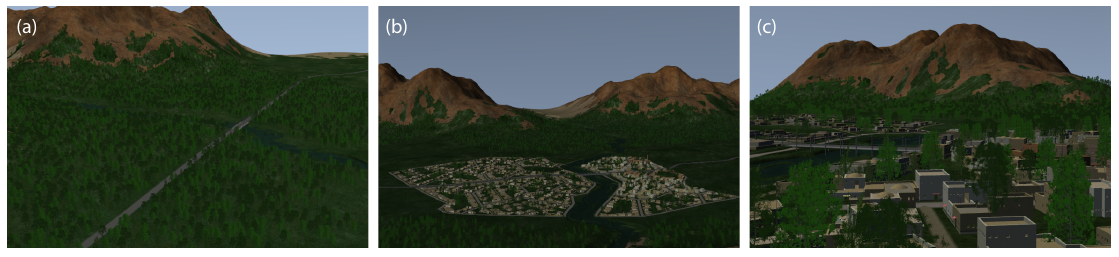
\includegraphics[width=15cm]{figuras/virtual_world.png}
	}
	{\Fonte{\cite{smelik2010}}}	
\end{figure}

Pode-se analisar a modelagem procedural de diferentes perspectivas: do poder expressivo à qualidade da produção, do tipo de interação do usuário à complexidade computacional, do grau de popularidade à área de aplicação \cite{smelik2014}, tais como terreno, vegetação, estradas, malhas fluviais, cidades e edifícios, os quais são o foco deste trabalho, sendo abordados na próxima seção.

\subsection{Edifícios}
\label{sec:edificios}

\citeonline{smelik2014} afirma que a geração procedural de edifícios é um dos campos mais desenvolvidos da modelagem procedural, havendo uma ampla utilização de algum sistema de reescrita formal, como \gls{L-Systems}, \textit{split grammars} ou \textit{shape grammars}, para gerar um modelo de construção 3D, a partir de uma representação 2D.

Outros métodos alternativos, por sua vez, tentam reconstruir as gramáticas a partir de um conjunto de dados do mundo real, conforme apresentado por \citeonline{nishida2018}, com a utilização de fotografias. No exemplo mostrado na Figura \ref{fig:fachada_foto}, a) dada uma imagem e a marcação da silhueta de um edifício, b) na primeira etapa, sua abordagem estima os parâmetros da câmera e gera uma gramática de massa do edifício. Em seguida, c) a imagem da fachada é retificada e d) a gramática da fachada é gerada. e) Para cada janela não-terminal, a melhor gramática de janela é selecionada. f) Finalmente, a gramática de saída é construída, e uma geometria 3D correspondente é gerada.

\begin{figure}[h!]
	\centering
	\captionsetup{width=15cm}
	\Caption{\label{fig:fachada_foto} Modelagem procedural a partir de uma imagem.}	
	\UFCfig{}{
		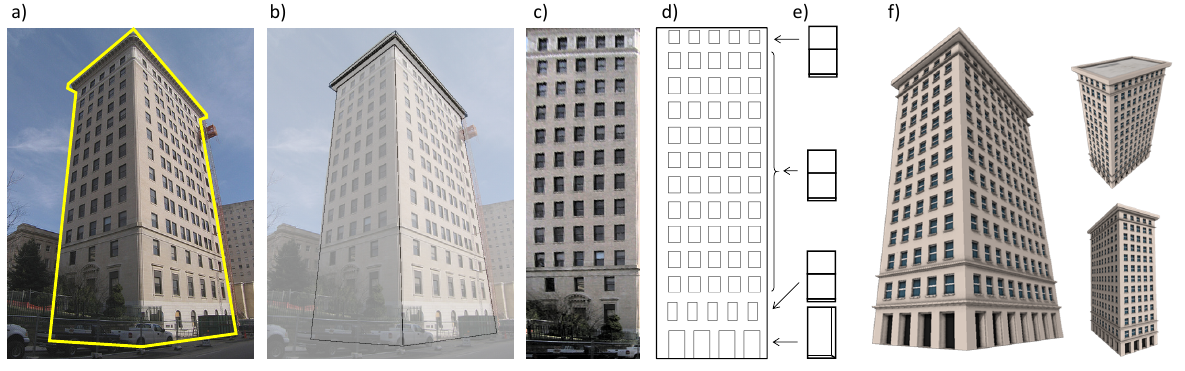
\includegraphics[width=15cm]{figuras/fachada_foto.png}
	}
	{\Fonte{\cite{nishida2018}}}	
\end{figure}

O processo de geração de edifícios por inteiro, ou seja, envolvendo fachadas e interiores, requer a utilização de métodos distintos para cada um dos casos. Na geração de fachadas, utilizam-se, geralmente, abordagens baseadas em gramáticas. Na geração de interiores, pode-se diferenciar entre a geração a partir da planta e a solução do \textit{layout} de móveis \cite{smelik2014}. O trabalho de \citeonline{leblanc2011} introduz um sistema para modelagem de edifícios completos, conforme ilustrado na Figura \ref{fig:interior}.

\begin{figure}[h!]
	\centering
	\captionsetup{width=15cm}
	\Caption{\label{fig:interior} Modelo de uma casa (à esquerda), com vista superior do primeiro andar (ao centro) e vista de dentro (à direita).}	
	\UFCfig{}{
		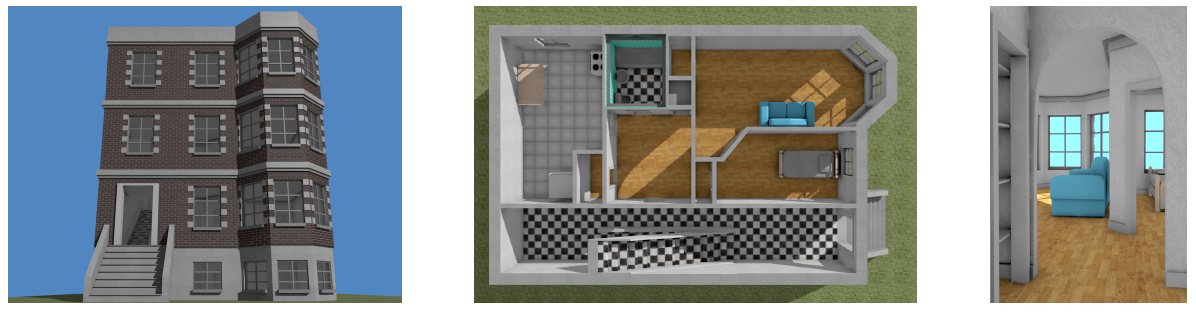
\includegraphics[width=15cm]{figuras/interior.png}
	}
	{\Fonte{\cite{leblanc2011}}}
\end{figure}

No contexto da geração procedural de edifícios, é importante conhecer o conceito de semântica, pois é ela que define se a estrutura dos modelos está organizada de maneira significativa, ou seja, condizente com exemplos arquiteturais do mundo real.

Conforme argumentado por \citeonline{musse2015}, para que a geometria tridimensional de um edifício seja gerada, um conjunto mínimo de dados deve ser fornecido pelo usuário, como uma lista de arestas e vértices para definir as paredes internas de cada cômodo, bem como as paredes externas do edifício, por exemplo. Na definição da parede, alguns pontos podem ser definidos para representar o centro das portas e janelas. Os quartos e suas paredes adjacentes podem receber um tipo, como cozinha, banheiro ou sala de estar. Algumas possíveis informações que podem ser definidas em uma entrada semântica são:

\begin{itemize}
    \item \textbf{Lista de materiais:} Categorizados por tipo de material, como parede externa, teto, vidro, e tipos de cômodo, que são utilizados para restringir os tipos de materiais usados para cada cômodo;
    
    \item \textbf{Estilos de janela:} Define as informações de dimensão (largura e altura), direção da abertura, profundidade da abertura, tipos de ambiente aos quais se aplica e materiais;
    
    \item \textbf{Estilos de portas:} Semelhantes aos estilos de janelas, de modo que diferentes características possam ser consideradas, como portas com topo arredondado, portas deslizantes, portas com painéis de vidro etc;
    
    \item \textbf{Estilos de telhado:} Tipos de telhado que podem ser usados na construção, definindo as dimensões, materiais e formas permitidas.
\end{itemize}

Uma definição semântica não é apenas uma definição de aparências, pois atribui sentido ao que está sendo criado, permitindo, por exemplo, informar que um material é mais resistente que outro, que um tipo específico de ambiente está associado a um tipo de janela característico, e que um determinado estilo arquitetônico exige que o telhado seja do tipo quadril \cite{musse2015}.

Nas próximas seções, por meio de uma abordagem cronológica, são apresentadas algumas das principais técnicas utilizadas na geração procedural de edifícios.

\section{L-Systems}
\label{sec:l_systems}

Os \gls{L-Systems} foram introduzidos por \citeonline{lindenmayer1968} para referenciar o estudo matemático da estrutura e desenvolvimento de organismos filamentosos. A ideia principal dos \gls{L-Systems} é alterar partes de um objeto inicial, aplicando sucessivas regras de substituição, com objetivo de gerar objetos mais elaborados.

Conforme descrito por \citeonline{simon2011}, uma forma é processada em duas etapas separadas. Na primeira, é realizado um processo de derivação a partir de um elemento inicial, o axioma. Na segunda, a \textit{string} pode ser interpretada geometricamente usando gráficos tartaruga. Nos gráficos tartaruga, a interpretação geométrica é obtida tomando cada símbolo como um desenho ou comando de movimento. Sintaticamente, um estado da tartaruga é dado pelo terceto $(x, y, \alpha)$, onde $(x, y)$ representa uma posição cartesiana, e $\alpha$ representa um ângulo que define a direção para qual a tartaruga está voltada. Dados um tamanho de passo $d$ e um ângulo $\beta$, a tartaruga pode responder aos seguintes comandos:

\vspace{0.5cm}

\begin{description}
    \item[] $F$ \quad Mover à frente uma distância $d$. Desta forma, o estado da tartaruga muda para $(x', y', \alpha)$, onde $x' = x + d cos(\alpha)$ e $y' = y + d sen(\alpha)$, então, uma linha entre $(x, y)$ e $(x', y')$ é desenhada;
    
    \item[] $+$ \quad Girar à esquerda por um ângulo $\beta$, fazendo o estado mudar para $(x, y, \alpha + \beta)$;
    
    \item[] $-$ \quad Girar à direita por um ângulo $\beta$, fazendo o estado mudar para $(x, y, \alpha - \beta)$;
    
    \item[] $[$ \quad \, Empilhar a posição atual na pilha de localização;
    
    \item[] $]$ \quad \, Ir para a posição gravada no topo da pilha e a desempilhar.
\end{description}

\vspace{0.5cm}

Historicamente, $F$, $+$, $-$, foram os primeiros símbolos introduzidos para modelar curvas fractais. Para modelar estruturas ramificadas, como plantas e árvores, os dois símbolos de colchetes foram adicionados, um para registrar a posição atual da tartaruga em uma pilha, e outro para recuperá-la \cite{simon2011}.

O floco de neve de Von Koch, representado na Figura \ref{fig:von_koch_snowflake}, é um exemplo clássico de curva fractal gerado por \gls{L-Systems}. O axioma é $\omega = F ++ F ++ F$, e a gramática é composta por uma única regra $F \rightarrow F - F ++ F - F$. Cada rotação corresponde a um ângulo $\alpha = 60$. A representação geométrica é mostrada para diferentes valores de $n$, que representa a quantidade de iterações da derivação \cite{simon2011}.
	
\begin{figure}[h!]
	\centering
	\captionsetup{width=15cm}
	\Caption{\label{fig:von_koch_snowflake} Geração do floco de neve de Von Koch utilizando \gls{L-Systems}.}	
	\UFCfig{}{
		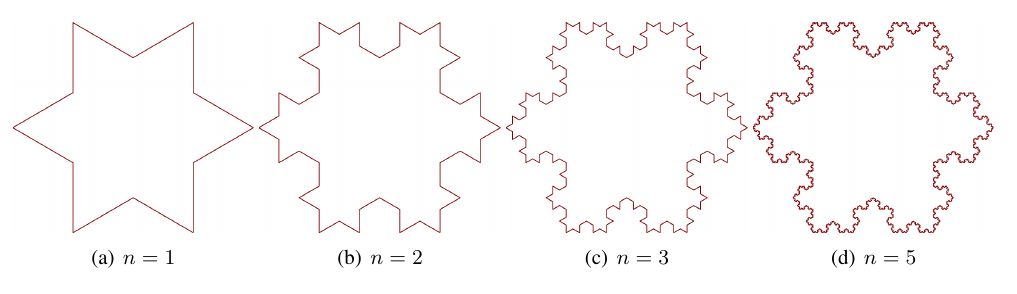
\includegraphics[width=15cm]{figuras/von_koch_snowflake.png}
	}
	{\Fonte{\cite{simon2011}}}	
\end{figure}

A Figura \ref{fig:algae} representa o sistema de uma alga, com intuito de ilustrar o uso dos colchetes. O axioma é $\omega = F$, e uma única regra $F \rightarrow F [+F] F [-F] [F]$ cria duas ramificações. São mostradas diferentes escalas de representação para um ângulo $\alpha = 25.7$ \cite{simon2011}. Da mesma maneira como no exemplo anterior, a representação geométrica é mostrada para diferentes valores de $n$. Além disso, por meio da extensão da gramática e das regras é possível obter resultados similares ao da Figura \ref{fig:l-system3d}.

\begin{figure}[h!]
	\centering
	\captionsetup{width=15cm}
	\Caption{\label{fig:algae} Geração de um modelo de alga utilizando \gls{L-Systems}.}	
	\UFCfig{}{
		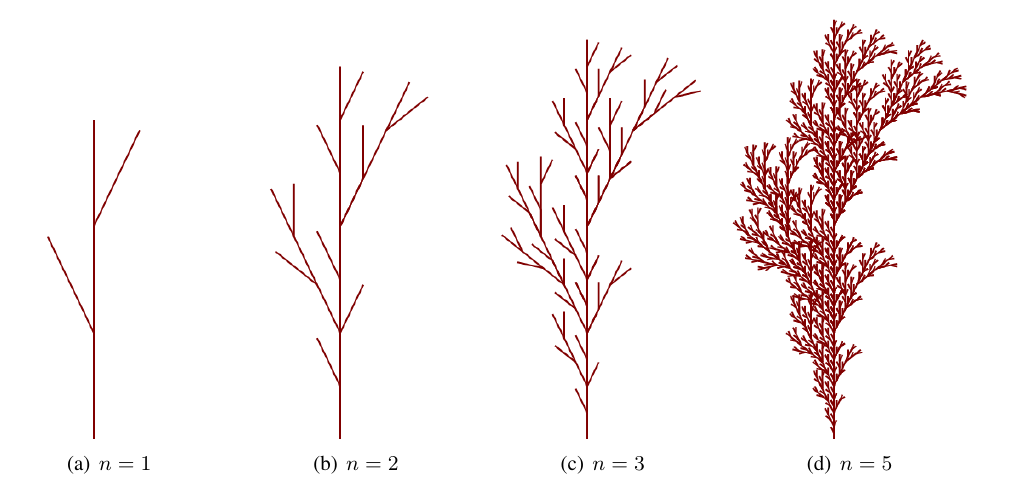
\includegraphics[width=15cm]{figuras/algae.png}
	}
	{\Fonte{\cite{simon2011}}}	
\end{figure}

\begin{figure}[h!]
	\centering
	\captionsetup{width=15cm}
	\Caption{\label{fig:l-system3d} Renderização tridimensional do modelo de uma \textit{Mycelis}.}	
	\UFCfig{}{
		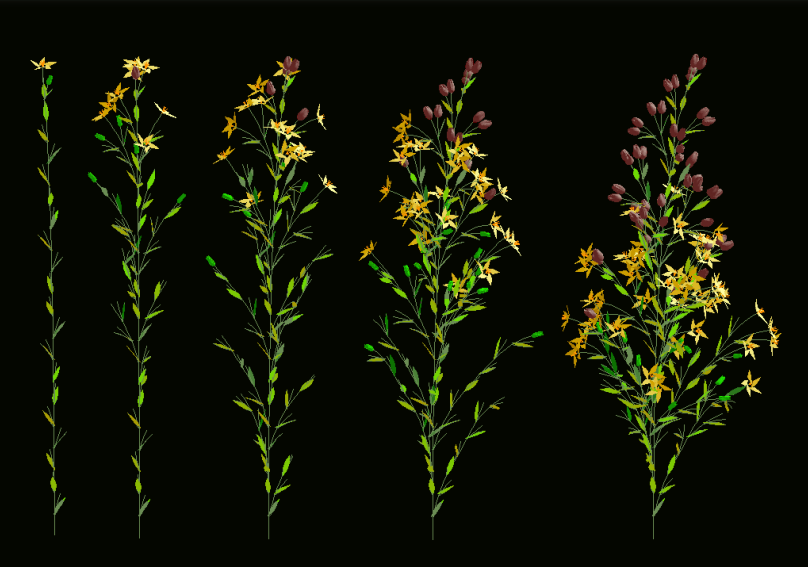
\includegraphics[width=14cm]{figuras/l-systems_plant.png}
	}
	{\Fonte{\cite{lindenmayer1996}}}	
\end{figure}

\section{Shape Grammars}
\label{sec:shape_grammars}

A ideia central das \textit{shape grammars} para criação de modelos 3D é começar com uma forma básica, como um cubo, e modificá-lo até que se pareça com o modelo desejado. Este procedimento é realizado aplicando-se várias operações à forma básica, como translação e rotação, ou outras mais complexas, como extrusão e divisão, resultando em um modelo mais elaborado. Para isso, no formalismo das \textit{shape grammars} é declarado um estado inicial (axioma), então, são atribuídos símbolos às formas e também são definidas regras de produção, que ditam como gerar símbolos e como aplicar as diferentes operações. Uma vez que as operações podem criar novas formas e o modelo resultante depende da aplicação de uma sequência de operações, geralmente, é utilizada uma árvore de derivação para armazenar tal sequência \cite{haubenwallner2016}.

\citeonline{stiny1972} introduziram as \textit{shape grammars} para representar a geração procedural de geometria. Por definição, uma \textit{shape grammar} é uma quádrupla $(V, L, R, \omega)$, onde:

\begin{itemize}
    \item $V$: é um conjunto finito de formas (vocabulário);
    \item $L$: é um conjunto finito de símbolos (rótulos);
    \item $R$: é um conjunto finito de regras no formato $\alpha \rightarrow \beta$, onde $\alpha$ e $\beta$ são formas rotuladas;
    \item $\omega$: é uma forma atômica chamada de axioma.
\end{itemize}

Uma regra $\alpha \rightarrow \beta$ se aplica à uma dada forma $\gamma$ se existe uma transformação $\delta$, tal que $\delta(\alpha)$ está contido em $\gamma$. Uma forma é composta de segmentos de linha rotulados. Após a aplicação de uma regra, a forma de saída é obtida substituindo-se na forma $\gamma$, a subforma $\delta(\alpha)$ por $\delta(\beta)$.

A Figura \ref{fig:greek_church} mostra um exemplo clássico de \textit{shape grammar}, criado por \citeonline{knight1995}, para descrever a planta de igrejas no formato de cruz grega. Contém uma única regra, transformando um retângulo em outros dois perpendiculares. A primeira linha mostra a única regra da gramática. A segunda linha mostra uma possível derivação em $n$ etapas, a partir de um retângulo como axioma.

\begin{figure}[h!]
	\centering
	\captionsetup{width=15cm}
	\Caption{\label{fig:greek_church} Gramática para gerar planta de igreja na forma de cruz grega.}	
	\UFCfig{}{
		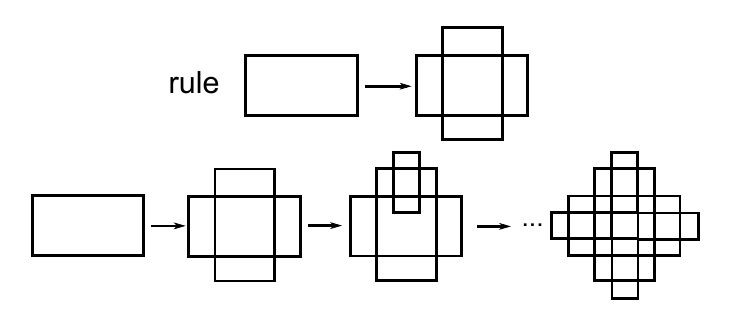
\includegraphics[width=10cm]{figuras/greek_cross_church.png}
	}
	{\Fonte{\cite{knight1995}}}	
\end{figure}

Desde a década de 1980, diferentes desenvolvimentos ampliaram as \textit{shape grammars} básicas para atender às diversas necessidades de geração de \textit{design}. A Figura \ref{fig:shape_grammars}, elaborada por \citeonline{gu2018}, mostra a cronologia das \textit{shape grammars} e seus desdobramentos.

\newpage

\begin{figure}[h!]
	\centering
	\captionsetup{width=15cm}
	\Caption{\label{fig:shape_grammars} Diagrama que descreve a cronologia das \textit{shape grammars}.}	
	\UFCfig{}{
		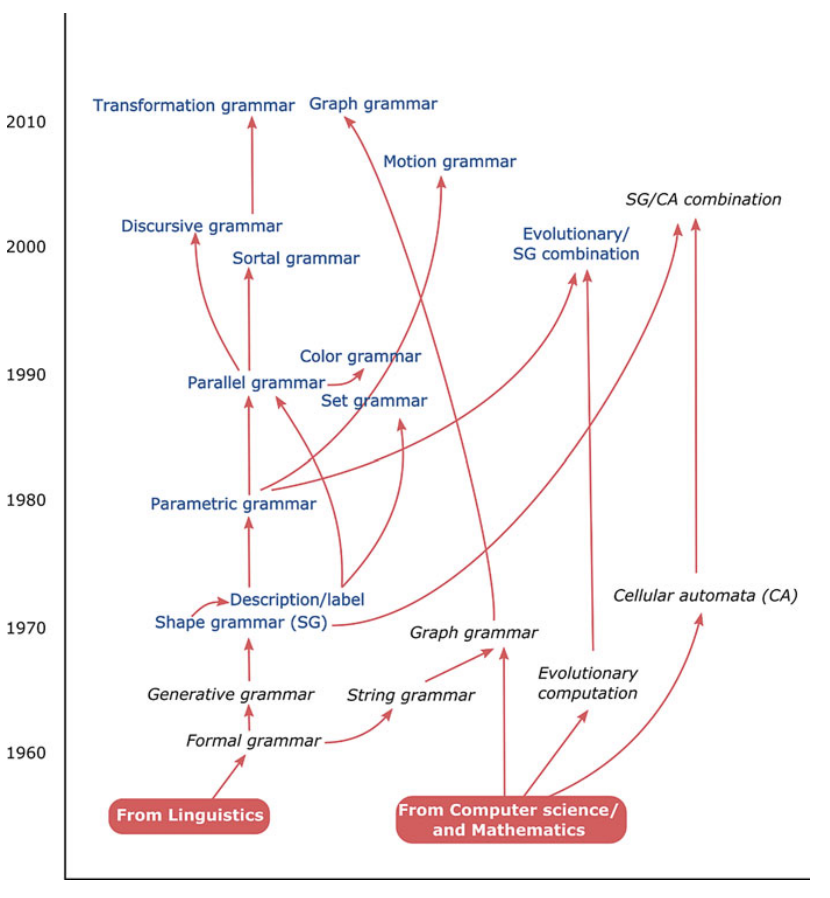
\includegraphics[width=15cm]{figuras/shape_grammars.png}
	}
	{\Fonte{\cite{gu2018}}}	
\end{figure}

\section{Split Grammar}
\label{sec:split_grammar}

As \textit{split grammars} foram introduzidas por \citeonline{wonka2003}, sendo utilizadas para modelagem procedural de construções, geralmente, fachadas de edifícios.

Uma descrição sucinta do formalismo é trazida por \citeonline{francisco2014}, na qual uma \textit{split grammar} é denotada por uma quádrupla $G = (N, T, \sigma , R)$, na qual $N$ representa o conjunto de símbolos não-terminais, $T$ representa o conjunto dos símbolos terminais, $\sigma \in R$ é a regra inicial e $R$ é o conjunto de regras. Cada símbolo terminal $\tau \in T$ está associado a um valor semântico para identificação do elemento da fachada que ele representa, como janela, parede, coluna etc. As regras $r \in R$, por sua vez, têm a forma $LHS \rightarrow RHS$, na qual $LHS \in N$ é um único símbolo não-terminal e $RHS$ é uma operação \textit{split} que aplicará as regras \textit{sucessoras} de $LHS$. 

\citeonline{francisco2014} explica que uma operação \textit{split} divide uma região geométrica horizontalmente ou verticalmente, e tem a seguinte configuração:

\vspace{0.5cm}

\begin{description}
    \item[] \qquad \qquad $split(axis) \rightarrow (repeat)\{\mu_0 s_0 : r_0, ... , \mu_n s_n : r_n \}$,
\end{description}

\vspace{0.5cm}

\noindent onde \textit{axis} representa o eixo em que a região do espaço será dividida; o símbolo \textit{repeat} é um modificador de regra opcional, o qual indica se as divisões devem ser aplicadas novamente, caso haja espaço sobrando, conforme exemplificado na Figura \ref{fig:split_exemplo_2}; $s_i$ representa o tamanho da divisão a ser aplicada na geometria que resultará em uma nova região retangular, na qual será aplicada a produção $r_i \in (N \cup T)$; e $\mu_i$ é o modificador da divisão, podendo ser três tipos:

\textbf{Absoluto:} Utilizado para criar uma nova região de tamanho igual a $s_i$ ao longo do eixo selecionado, se houver espaço suficiente.

\textbf{Aproximado:} Força a nova região a ter tamanho, pelo menos, $s_i$, sendo representado na gramática pelo símbolo $\sim$. Ao final de todas as divisões da operação \textit{split}, se ainda existir espaço sobrando, as regiões marcadas com este modificador aumentarão de tamanho por um número proporcional a $s_i$, fazendo com que toda a região passada como entrada para a regra seja ocupada.

\textbf{Relativo:} Seja $t$ o tamanho da forma inicial, assim, o tamanho da nova região a ser criada será $s_i * t$. Para utilização de toda a região na qual uma regra é aplicada, é preciso garantir que a soma dos tamanhos do \textit{split} com modificadores relativos seja igual a $1,0$. Na gramática, é representado pelo símbolo $'$.

\citeonline{francisco2014} pontua que numa única operação \textit{split} é permitido que cada divisão possua um modificador diferente. Na Figura \ref{fig:split_exemplo_1}, por exemplo, é mostrado o uso dos modificadores absoluto e aproximado em uma mesma operação, onde \textit{UpperFloors} e \textit{GroundFloors} representam símbolos não-terminais. A Figura \ref{fig:split_exemplo_2}, por sua vez, mostra o uso do \textit{repeat}.

\begin{figure}[h!]
	\centering
	\captionsetup{width=15cm}
	\Caption{\label{fig:split_exemplo_1} Exemplo de \textit{split} com o modificador aproximado ($\sim$). A regra que leva a essa configuração é $Facade \rightarrow split(Y){4 : GroundFloor, \sim 1 : UpperFloors}$.}	
	\UFCfig{}{
		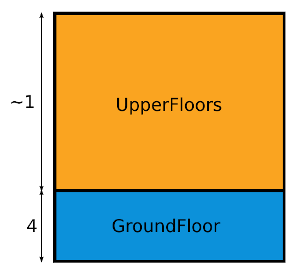
\includegraphics[width=7cm]{figuras/split_exemplo_1.png}
	}
	{\Fonte{\cite{francisco2014}}}	
\end{figure}

\begin{figure}[h!]
	\centering
	\captionsetup{width=15cm}
	\Caption{\label{fig:split_exemplo_2} Exemplo de \textit{split} com repetição. A regra que leva a essa derivação é \\ $S \rightarrow repeat split(X){1 : A, 3 : B, 2 : C}$.}	
	\UFCfig{}{
		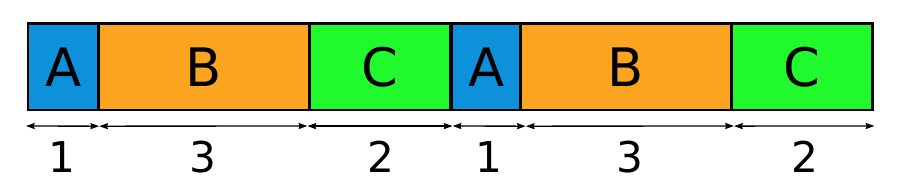
\includegraphics[width=10cm]{figuras/split_exemplo_2.png}
	}
	{\Fonte{\cite{francisco2014}}}	
\end{figure}

Conforme argumentado por \citeonline{francisco2014}, a partir de uma palavra de uma dada gramática, é possível representar uma fachada por meio de uma árvore de derivação, onde cada nó desta árvore associa uma região retangular do espaço a um símbolo da gramática $\varphi \in (T \cup N)$, de modo que os nós intermediários particionam essa região pela aplicação de uma regra $\eta \in R$, e os nós folhas, por sua vez, representam os elementos atômicos que compõem a fachada, como janelas, portas e paredes, identificados pelos símbolos terminais $\tau \in T$ associados a eles. Para exemplificar esta ideia, a Figura \ref{fig:arvore_derivacao_split} representa a árvore de derivação correspondente à fachada da Figura \ref{fig:fachada_split}.

\begin{figure}[h!]
	\centering
	\captionsetup{width=15cm}
	\Caption{\label{fig:arvore_derivacao_split} Árvore de derivação.}	
	\UFCfig{}{
		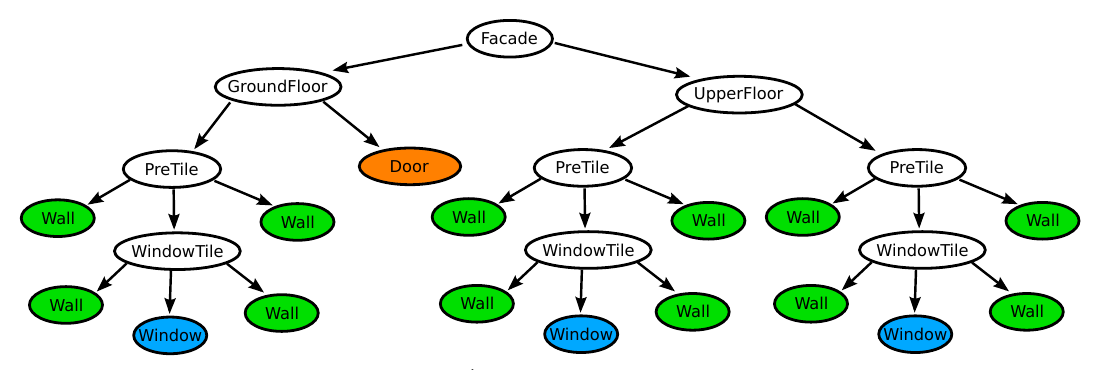
\includegraphics[width=15cm]{figuras/arvore_derivacao_split.png}
	}
	{\Fonte{\cite{francisco2014}}}	
\end{figure}

\begin{figure}[h!]
	\centering
	\captionsetup{width=15cm}
	\Caption{\label{fig:fachada_split} Fachada.}	
	\UFCfig{}{
		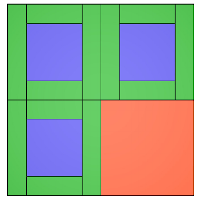
\includegraphics[width=6cm]{figuras/fachada_split.png}
	}
	{\Fonte{\cite{francisco2014}}}	
\end{figure}

\newpage

\section{CGA Shape}
\label{sec:cga}

A \textit{CGA Shape} foi proposta por \citeonline{muller2006} para geração procedural de modelos arquiteturais, trazendo melhorias em relação às \textit{split grammars}. Como contribuição, introduz regras de divisão com repetição, regras de redimensionamento e regras de divisão de componentes. A notação da gramática e as regras gerais para adicionar, redimensionar, transladar e rotacionar as formas são estendidas dos \gls{L-Systems}, mas voltadas para a modelagem de arquiteturas.

Com objetivo de formalizar a \textit{CGA Shape}, \citeonline{muller2006} apresenta as seguintes definições:

\textbf{Forma:} Uma forma consiste em um símbolo (\textit{string}), atributos geométricos e atributos numéricos. As formas são identificadas por seus símbolos, sendo um terminal $\alpha \in \Sigma$ ou um não-terminal $\beta \in V$. As formas correspondentes são chamadas de formas terminais e formas não-terminais. Os atributos geométricos mais importantes são a posição $P$, três vetores ortogonais $X$, $Y$ e $Z$, que descrevem um sistema de coordenadas, e um vetor de tamanho $S$. Em conjunto, tais atributos definem o escopo, ou seja, uma caixa delimitadora orientada no espaço, conforme mostrado na Figura \ref{fig:cga_shape}.

\begin{figure}[h!]
	\centering
	\captionsetup{width=15cm}
	\Caption{\label{fig:cga_shape} Representação geométrica da \textit{CGA Shape}. Esquerda: definição de uma \textit{box} no espaço contendo uma forma primitiva. Direita: Modelo simples de uma construção usando três primitivas.}
	\UFCfig{}{
		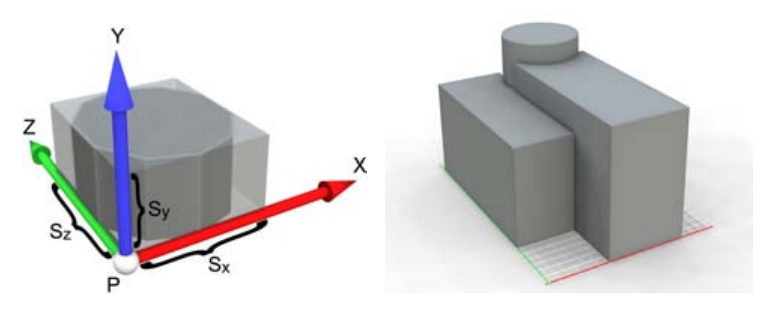
\includegraphics[width=13cm]{figuras/cga_shape.png}
	}
	{\Fonte{\cite{muller2006}}}	
\end{figure}

\textbf{Processo de produção:} Um conjunto finito de formas básicas define uma configuração. O processo de produção pode começar com uma configuração arbitrária de formas $A$, chamada de axioma, e prossegue da seguinte maneira: (1) Selecione uma forma ativa com o símbolo $B$ no conjunto; (2) escolha uma regra de produção com $B$ no lado esquerdo para computar um sucessor para $B$, ou seja, um novo conjunto de formas $BNEW$; (3) marque a forma $B$ como inativa e adicione as formas $BNEW$ à configuração e continue com a etapa (1). Finalmente, o processo de produção termina quando não existirem mais não-terminais na configuração. Dependendo do algoritmo de seleção na etapa (1), a árvore de derivação pode ser explorada tanto em profundidade quanto em largura. Para isso, é atribuída uma prioridade à todas as regras de acordo com o detalhe representado pela forma, assim, para obter uma derivação em largura, seleciona-se a forma com a regra de maior prioridade na etapa (1). É importante pontuar que as formas não são excluídas, mas sim marcadas como inativas, após serem substituídas. Isso permite a consulta na hierarquia de formas como um todo, e não apenas na configuração ativa.

\textbf{Notação:} As regras de produção são definidas da seguinte maneira:

\vspace{0.5cm}

\begin{description}
    \item[] \qquad \qquad $id: predecessor : cond \rightsquigarrow successor : prob$,
\end{description}

\vspace{0.5cm}

\noindent onde \textit{id} é um identificador único para a regra, $predecessor \in V$ é um símbolo que identifica uma forma que deve ser substituída por \textit{sucessor}, e \textit{cond} é uma expressão lógica que deve ser avaliada como verdadeira para que a regra seja aplicada. Uma regra, por sua vez, é selecionada com probabilidade \textit{prob}. Por exemplo, a regra

\vspace{0.5cm}

\begin{description}
    \item[] \qquad \qquad  $1: fac(h): h > 9 \rightsquigarrow floor(h/3) floor(h/3) floor(h/3)$
\end{description}

\vspace{0.5cm}

\noindent substitui a forma de \textit{fac} por três formas \textit{floor}, se o parâmetro $h$ é maior que 9.

\textbf{Regras do escopo:} Regras utilizadas para modificar as formas, onde $T(t_x, t_y, t_z)$ é um vetor de translação que é adicionado ao escopo da posição $P$; $R_x(angle)$, $R_y(angle)$ e $R_z(angle)$ gira o respectivo eixo do sistema de coordenadas; e $S(s_x, s_y, s_z)$ define o tamanho do escopo. Os símbolos $[$ e $]$ são utilizados, respectivamente, para empilhar e desempilhar o escopo atual na pilha, similar aos \gls{L-Systems}. Qualquer símbolo não-terminal $ \beta \in V$ na regra é criado com o escopo atual. Da mesma maneira, o comando $I(objId)$ adiciona uma instância de uma primitiva geométrica com identificador \textit{objId}. Objetos padrões incluem um cubo, um quadrângulo e um cilindro, contudo, qualquer modelo tridimensional pode ser usado. A seguinte regra representa o \textit{design} do modelo de massa apresentado na Figura \ref{fig:cga_shape}:

\vspace{0.5cm}

\begin{description}
    \item[] \qquad \qquad $1: A \rightsquigarrow [ T(0,0,6) S(8,10,18) I("cube") ]$
    \item[] \qquad \qquad \, \, \, $T(6,0,0) S(7,13,18) I("cube") T(0,0,16) S(8,15,8) I("cylinder")$.
\end{description}

\vspace{0.5cm}

\textbf{Regra de divisão básica}: Divide o escopo atual ao longo de um eixo. Por exemplo, considere a regra para dividir a fachada da Figura \ref{fig:cga_shape_exemplo} em quatro andares e uma saliência:

\vspace{0.5cm}

\begin{description}
    \item[] \qquad \qquad $1: fac \rightsquigarrow Subdiv("Y",3.5,0.3,3,3,3)\{ floor | ledge | floor | floor | floor \}$.
\end{description}

\vspace{0.5cm}

O primeiro parâmetro descreve o eixo dividido, sendo "$X$", "$Y$" \, ou "$Z$", e os parâmetros restantes descrevem os tamanhos da divisão. Entre os delimitadores $\{$ e $\}$ é fornecida uma lista de formas, separadas por $|$. Além disso, são utilizadas regras de divisão semelhantes para dividir ao longo de vários eixos, como "$XY$", "$XZ$", "$YZ$" \, ou "$XYZ$".

\begin{figure}[h!]
	\centering
	\captionsetup{width=15cm}
	\Caption{\label{fig:cga_shape_exemplo} Aplicação das regras da \textit{CGA Shape}. À esquerda: Um \textit{design} básico de fachada. À direita: Uma divisão simples que poderia ser usada para os três andares superiores.}	
	\UFCfig{}{
		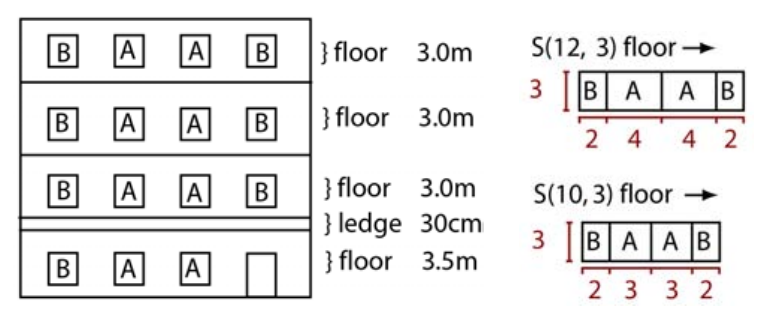
\includegraphics[width=12cm]{figuras/cga_shape_exemplo.png}
	}
	{\Fonte{\cite{muller2006}}}	
\end{figure}

\textbf{Regras de redimensionamento:} Nem todas as partes da arquitetura são redimensionadas igualmente, por isso, é possível distinguir entre valores absolutos, que não redimensionam, e valores relativos, que redimensionam. Os valores são considerados absolutos por padrão, então, para denotar valores relativos é utilizada a letra $r$, conforme mostrado no exemplo a seguir:

\vspace{0.5cm}

\begin{description}
    \item[] \qquad \qquad $1: floor \rightsquigarrow Subdiv("X",2,1r,1r,2) \{ B | A | A | B \}$,
\end{description}

\vspace{0.5cm}

\noindent no qual os valores relativos $r_i$ são substituídos como $r_i * (Scope.sx - \sum abs_i / \sum r_i)$, onde $Scope.sx$ representa o tamanho de $x\mbox{-}length$ do escopo atual.

\textbf{Repetição:} Para permitir mudanças em maior escala nas regras de divisão, geralmente, é interessante incluir um elemento específico lado a lado. Por exemplo:

\vspace{0.5cm}

\begin{description}
    \item[] \qquad \qquad $1: floor \rightsquigarrow Repeat("X",2) \{ B \}$.
\end{description}

\vspace{0.5cm}

Neste caso, enquanto houver espaço, \textit{floor} será revestido com tantos elementos do tipo $B$, ao longo do eixo x do escopo. O número de repetições é calculado a partir do valor de $repetitions = \ceil{Scope.sx/2}$, então, o tamanho real do elemento é ajustado de acordo.

\textbf{Divisão de componentes:} Esta nova operação permite dividir o escopo em formas de dimensões menores, conforme exemplificado no comando a seguir:

\vspace{0.5cm}

\begin{description}
    \item[] \qquad \qquad $1: a \rightsquigarrow Comp(type, param) \{ A | B | ... | Z \}$,
\end{description}

\vspace{0.5cm}

\noindent onde \textit{type} identifica o tipo de divisão do componente com os parâmetros associados \textit{param}, se existirem. Por exemplo, $Comp("faces") \{A\}$ cria uma forma com o símbolo $A$ para cada face da forma tridimensional original. Da mesma maneira, $Comp("edges") \{B\}$ e $Comp("vertices") \{C\}$ são usados para dividir arestas e vértices, respectivamente. Para acessar apenas os componentes selecionados são utilizados comandos como $Comp("edge", 3) \{A\}$ para criar uma forma $A$ alinhada com a terceira aresta do modelo, ou $Comp("side faces) \{B\}$ para acessar as faces laterais de um cubo ou cilindro poligonal. Para codificar formas de menor dimensão, são utilizados escopos cujos eixos têm tamanho diferente de zero. Para voltar à dimensões superiores, pode-se utilizar o comando $S$ com um valor não-nulo na dimensão correspondente, por exemplo, para extrudar uma forma de face ao longo de sua normal e, portanto, transformá-la em uma forma volumétrica.

\subsection{Aplicações}
\label{sec:cga_exemplos}

Para demonstrar a aplicação da \textit{CGA Shape}, \citeonline{muller2006} apresenta exemplos nos seguintes contextos:

\textbf{Prédios comerciais:} Inicialmente, é definido um conjunto de regras para gerar vários modelos com base em uma gramática estocástica. O axioma da gramática é uma forma bidimensional, representando um lote de construção. As regras, por sua vez, funcionam da seguinte maneira: na regra \ref{itm:cga_rule_1}, o lote é extrudado com altura definida pelo valor de $building\_height$, utilizando um comando de tamanho para produzir uma forma tridimensional. Essa forma é, então, dividida em duas formas menores. Uma forma volumétrica (fachadas), que é o maior sólido no modelo, e uma forma que, posteriormente, será dividida em duas asas laterais. Essa divisão é realizada pela regra \ref{itm:cga_rule_2}, que também gera uma lacuna entre as asas laterais, criando, assim, um formato de U. A regra \ref{itm:cga_rule_3} mostra o uso de regras estocásticas para gerar uma variedade de modelos com diferentes configurações. Além disso, são utilizadas combinações de números aleatórios e seleção estocástica de regras, para criar uma variedade de formatos de asa lateral com diferentes alturas e larguras. A regra \ref{itm:cga_rule_4} é a transição para a modelagem de fachada, permitindo que em estágios posteriores possam ser adicionadas portas e janelas, por exemplo. Um modelo gerado a partir destas quatro regras é ilustrado na Figura \ref{fig:cga_shape_models}.

\vspace{0.5cm}

\begin{enumerate}
    \item \label{itm:cga_rule_1} $lot \rightsquigarrow S(1r,building\_height,1r)$ \\
        \qquad \qquad $Subdiv("Z",Scope.sz*rand(0.3,0.5),1r)\{ facades | sidewings \}$
    \item \label{itm:cga_rule_2} $sidewings \rightsquigarrow $ \\
        \qquad \qquad $Subdiv("X",Scope.sx*rand(0.2,0.6),1r)\{ sidewing | \epsilon \}$ \\
        \qquad \qquad $Subdiv("X",1r,Scope.sx*rand(0.2,0.6))\{ \epsilon | sidewing \}$
    \item \label{itm:cga_rule_3} $sidewing$ \\
        \qquad \qquad $\rightsquigarrow S(1r,1r,Scope.sz*rand(0.4,1.0)) facades : 0.5$ \\
        \qquad \qquad $\rightsquigarrow S(1r,Scope.sy*rand(0.2,0.9),Scope.sz*rand(0.4,1.0))
    facades : 0.3$ \\
        \qquad \qquad$ \rightsquigarrow \epsilon : 0.2$
    \item \label{itm:cga_rule_4} $facades \rightsquigarrow Comp("sidefaces")\{ facade \}$
\end{enumerate}

\vspace{0.5cm}

\begin{figure}[h!]
	\centering
	\captionsetup{width=15cm}
	\Caption{\label{fig:cga_shape_models} Variações estocásticas de modelos de edifícios.}	
	\UFCfig{}{
		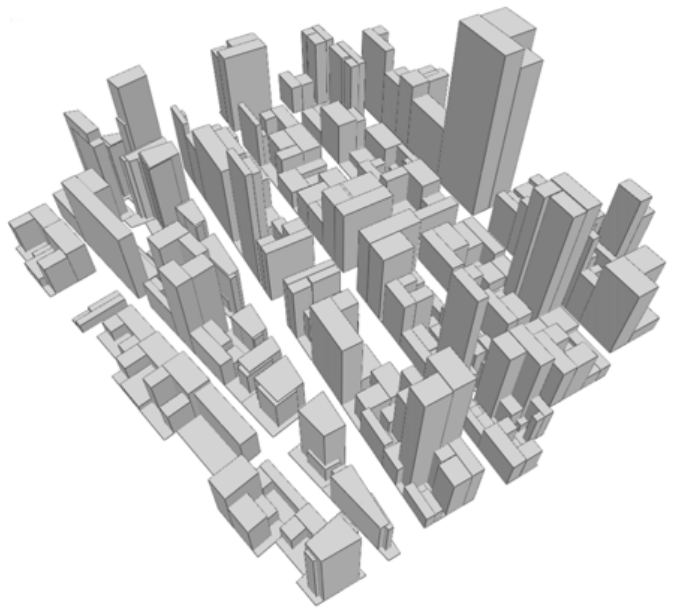
\includegraphics[width=10cm]{figuras/cga_shape_models.png}
	}
	{\Fonte{\cite{muller2006}}}	
\end{figure}

\newpage

\textbf{Residências:} \textit{shape grammars} e consulta de formas, em conjunto, podem ser utilizadas na geração de ambientes urbanos, conforme mostrado na Figura \ref{fig:cga_houses}. A gramática, neste caso, usa a seguinte estratégia: dividir as bordas da propriedade com uma divisão de componentes e colocar arbustos perto da cerca; dividir a propriedade para modelar o jardim da frente, o quintal e a construção principal; gerar uma calçada e colocar árvores em intervalos regulares ao lado da rua; e, por fim, gerar uma calçada conectada à porta da garagem, e uma via conectada à porta de entrada.

\begin{figure}[h!]
	\centering
	\captionsetup{width=15cm}
	\Caption{\label{fig:cga_houses} Diferentes construções em um ambiente suburbano.}	
	\UFCfig{}{
		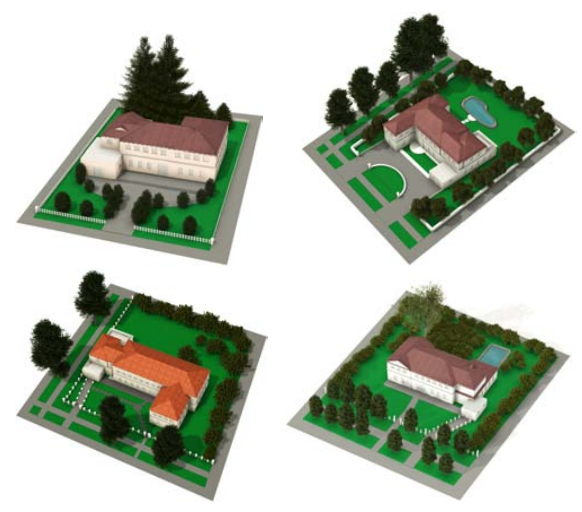
\includegraphics[width=8cm]{figuras/cga_family_houses.png}
	}
	{\Fonte{\cite{muller2006}}}	
\end{figure}

\section{CGA++}
\label{sec:cga++}

A \textit{CGA++} foi introduzida por \citeonline{schwarz2015} como sendo uma evolução natural da \textit{CGA Shape}, com o objetivo de superar algumas limitações existentes na modelagem procedural de arquiteturas, tais como:

\vspace{0.5cm}

\begin{enumerate}
    \item \label{itm:limitation_1} A coordenação do refinamento de decisões através de múltiplas formas não é diretamente suportada. Assim, qualquer decisão que afete várias formas deve ser tomada, o mais tardar, no ponto onde as linhagens dessas formas divergem e, portanto, antes que essas formas existam, para em seguida, ser transmitida nas regras;

    \item \label{itm:limitation_2} Normalmente, não são possíveis operações envolvendo múltiplas formas, ou seja, não podem ser expressas nem operações \textit{booleanas}, como formar a interseção de duas formas, nem montar uma forma a partir de várias outras, por exemplo;

    \item \label{itm:limitation_3} Informações contextuais, geralmente, não estão disponíveis, o que impede considerar informações de outras formas, algo necessário para determinados objetivos de modelagem, tal como o alinhamento;

    \item \label{itm:limitation_4} O suporte para explorar múltiplas formas é inexistente. Em particular, não é possível gerar uma derivação de dentro de outra derivação e consultar ou incorporar o resultado.
\end{enumerate}

\vspace{0.5cm}

Tendo em vista estas dificuldades, \citeonline{schwarz2015} apresentam dois novos recursos com a \textit{CGA++}. 

Em primeito lugar, as formas ficam diretamente expostas na gramática, permitindo que formas individuais sejam identificadas de maneira única, bem como transmitidas e armazenadas como valores. Assim, as operações podem tomar formas como argumentos, permitindo operações \textit{booleanas} em múltiplas formas, endereçando \ref{itm:limitation_2}. Além disso, torna-se possível acessar, percorrer e consultar a árvore de formas gerada pelo processo de derivação, o que facilita a obtenção de informações contextuais genéricas, endereçando \ref{itm:limitation_3}. Também é importante ressaltar que árvores de formas temporárias podem ser criadas instantaneamente em tempo de execução, por exemplo, gerando uma nova derivação ou invocando uma função em uma árvore existente, permitindo, assim, que alternativas possam ser buscadas e formas auxiliares possam ser utilizadas diretamente de dentro de uma gramática, endereçando \ref{itm:limitation_4}. 

Em segundo lugar, juntamente com o dispositivo linguístico de eventos, é fornecido um mecanismo de agrupamento dinâmico e facilidade de sincronização, permitindo a coordenação entre um grupo de formas, como a troca de informações ou o estabelecimento de uma decisão coerente sobre como proceder individualmente, endereçando \ref{itm:limitation_1}. Além disso, os eventos podem ser usados para influenciar a ordem do processo de derivação, garantindo a disponibilidade de todas as formas necessárias ao realizar uma consulta contextual, endereçando \ref{itm:limitation_3}.

\citeonline{schwarz2015} afirmam que estes novos recursos são bastante poderosos e possibilitam uma ampla gama de novas aplicações, permitindo ainda:

\begin{itemize}
    \item Operações que utilizam diversas formas como entrada, tais quais operações \textit{booleanas}, além de decomposição, refinamento e recomposição de fluxos de trabalho;

    \item Coordenação genérica através de várias formas;

    \item Estabelecimento e consulta de contextos genéricos, como adjacência espacial de formas.
\end{itemize}

\subsection{Especificações}
\label{sec:especificacoes}

Segundo \citeonline{schwarz2015}, uma ideia chave para superar as limitações descritas anteriormente, na Seção \ref{sec:cga++}, é tornar as formas e a árvore de formas disponíveis na gramática. Com o processo de derivação definindo a árvore de formas, cada forma que é gerada durante a derivação corresponde a um nó desta árvore, o que identifica ainda mais a subárvore que tem raiz neste nó. Assim, os termos \textit{forma}, \textit{nó}, e \textit{(sub)árvore} oferecem visualizações diferentes da mesma entidade. Uma vez que tal interpretação é adotada, as entidades são expostas diretamente na linguagem.

\citeonline{schwarz2015} argumentam que a \textit{CGA++} oferece diversas opções para fazer referência a uma forma existente. Além de consultar a árvore de formas, as formas em um corpo de regra podem ser convenientemente acessadas por nome. Uma vez que a forma é identificada, ela pode participar livremente nas expressões; em particular, pode ser usada como argumento para funções e operações. Como um simples exemplo instrutivo, a gramática na Figura \ref{fig:cga++_exemplo_1} demonstra a operação \textit{booleana} \texttt{minus}, que modifica a forma atual subtraindo dela uma dada forma, podendo ser empregada para evitar a sobreposição de áreas na construção.

\begin{figure}[h!]
	\centering
	\captionsetup{width=15cm}
	\Caption{\label{fig:cga++_exemplo_1} Exemplo ilustrativo do uso da \textit{CGA++}.}	
	\UFCfig{}{
		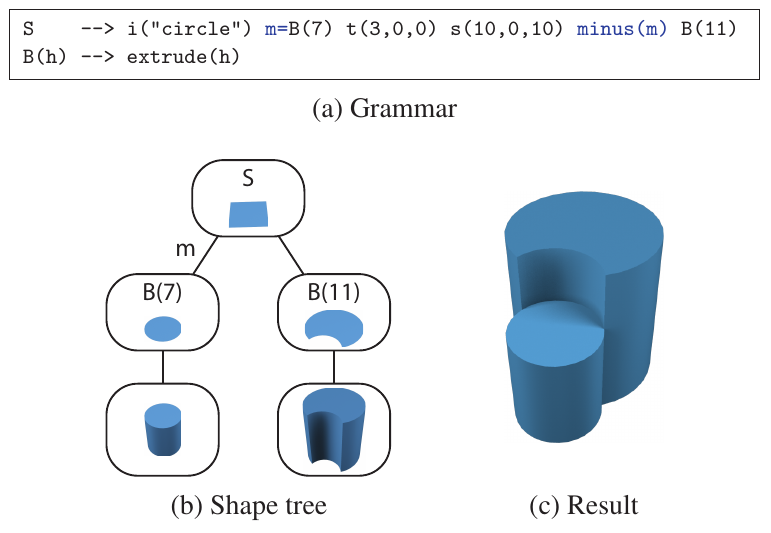
\includegraphics[width=13cm]{figuras/cga++_exemplo_1.png}
	}
	{\Fonte{\cite{schwarz2015}}}	
\end{figure}

\newpage

Com objetivo de definir operações e conceitos importantes para entendimento da \textit{CGA++}, \citeonline{schwarz2015} apresentam as seguintes especificações:

\textbf{Consultando a árvore de formas:} A \textit{CGA++} oferece funções para navegar, arbitrariamente, na árvore de formas (Figura \ref{fig:cga++_arvore}). Neste contexto, dado um nó, tanto seu pai quanto sua lista de filhos podem ser consultados. Além disso, também existem funções que retornam todos os nós folha de uma dada subárvore, ou uma lista de todos os nós enumerados de acordo com uma ordem de percorrimento especificada. A ausência de um nó é denotada por \texttt{null} nas gramáticas. Para fazer referência a um nó filho rotulado, o operador de acesso associativo à esquerda \textbf{\texttt{::}} pode ser utilizado, o qual leva um nó em seu lado esquerdo e um rótulo em seu lado direito. Uma consulta na árvore de formas pode ser realizada através de atributos, permitindo abstrair a estrutura exata da árvore, o que facilita a localização de uma determinada forma com base em algum critério. Na \textit{CGA++}, cada forma pode ter um número arbitrário de atributos, que podem ser definidos e recuperados. Um atributo é identificado por um nome e seu valor pode ser de qualquer tipo compatível com a linguagem, incluindo uma forma.

\begin{figure}[h!]
	\centering
	\captionsetup{width=15cm}
	\Caption{\label{fig:cga++_arvore} Algumas das opções de navegação da árvore, onde \texttt{a} e \texttt{b} são valores representando as formas dos nós 1 e 2, respectivamente, enquanto \texttt{X} e \texttt{Y} são rótulos.}	
	\UFCfig{}{
		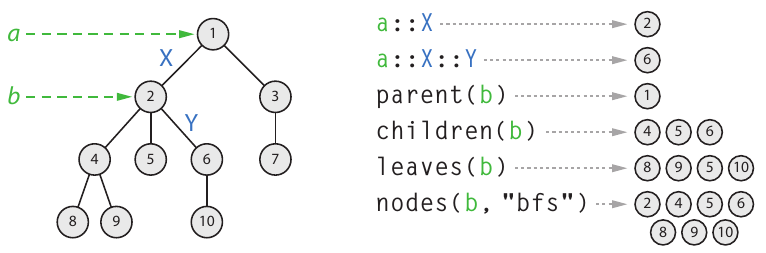
\includegraphics[width=15cm]{figuras/cga++_arvore.png}
	}
	{\Fonte{\cite{schwarz2015}}}
\end{figure}

\textbf{Construindo novas formas:} Para gerar um novo processo de derivação dentro do atual, utiliza-se o construto $<actions>(base)$, que possibilita criar uma nova árvore de (sub)formas. Empregando a forma identificada por \textit{base} como forma inicial, as ações especificadas são executadas e a árvore resultante é retornada. Se o argumento \textit{base} for omitido, a forma atual será usada.

\textbf{Funções:} Uma nova árvore de formas é produzida por várias funções internas, podendo ser derivada de uma ou mais (sub)árvores de entrada. Um conjunto dessas funções se preocupa, principalmente, com a modificação de formas. Por exemplo, a função \texttt{transformScope}\textit{(source, target)} retorna uma cópia da origem, onde os escopos de todos os nós estão sujeitos à transformação, fazendo o escopo do nó raiz idêntico ao escopo de destino, ou seja, ajustando a origem no destino. Para outras operações, são fornecidas funções que tomam uma forma a ser manipulada como argumento e retornam o resultado como uma nova forma. Como exemplo, \texttt{t}$(tree, \Delta x, \Delta y, \Delta z)$ translada os escopos de todos os nós da árvore especificada pelo deslocamento dado. Também existem funções para operações de subdivisão, cada uma retornando uma lista com todas as partes resultantes. Outro conjunto de funções se concentra na manipulação da estrutura das árvores. Além das funções elementares para criar uma nova árvore com determinados filhos, e para adicionar, remover ou substituir subárvores de uma determinada árvore, são oferecidas funções de alto nível de reescrita de árvore, o que permite a poda de subárvores, bem como o refinamento de nós folha, por meio da invocação de uma regra fornecida para eles.

\textbf{Formas recuperáveis:} As formas recuperáveis servem como nós indicadores para onde a derivação deve ser continuada em estágios futuros. Para criação de uma forma recuperável utiliza-se \texttt{?}$name(arg_0, ...)$, registrando a forma atual e os argumentos fornecidos, sendo, basicamente, um nó (forma) com atributos especiais. A função \texttt{continue}$(tree, name_0 = rule_0, ...)$ invoca a regra $rule_i$ para todas as formas recuperáveis na árvore fornecida, cujo nome corresponda a $name_i$, usando os argumentos associados à respectiva forma recuperável, e retorna uma árvore adequadamente refinada. A Figura \ref{fig:formas_recuperaveis} mostra um exemplo, onde duas árvore de formas parciais são construídas, e a que se mostra como a melhor opção é, então, completada pelo refinamento das formas recuperáveis da árvore adequada. A regra \texttt{Parcel} explora dois esquemas de desenvolvimento alternativos, primeiro, construindo parcialmente as duas árvores de formas correspondentes, depois, atribuindo às variáveis \texttt{a} e \texttt{b} para uso subsequente. As regras \texttt{DesignA} e \texttt{DesignB}, em última análise, geram formas \texttt{Footprint} e as extrudam, produzindo massas de construção, cujo refinamento é adiado pela emissão de uma forma recuperável \texttt{?Mass}. Empregando a função \texttt{V}, que soma os volumes das formas (folhas) de uma determinada árvore, a regra \texttt{Parcel}, então, determina a árvore com o maior volume de massa total, e continua o refinamento em suas formas recuperáveis usando a regra \texttt{Mass1} ou \texttt{Mass2}, respectivamente. Por fim, a árvore de formas resultante é incorporada por meio da utilização do \texttt{include}.

\begin{figure}[h!]
	\centering
	\captionsetup{width=15cm}
	\Caption{\label{fig:formas_recuperaveis} Exemplo do uso de formas recuperáveis. Considera dois \textit{designs} diferentes, escolhe aquele que resulta no maior volume de massa total e continua sua derivação para desenvolver as massas em edifícios detalhados.}	
	\UFCfig{}{
		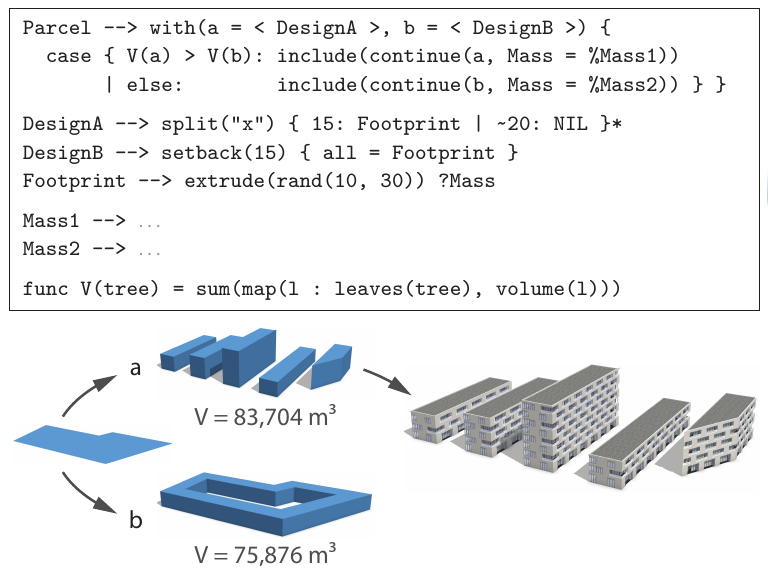
\includegraphics[width=12cm]{figuras/exemplo_formas_recuperaveis.png}
	}
	{\Fonte{\cite{schwarz2015}}}
\end{figure}

\citeonline{schwarz2015} também introduziram os eventos, que servem como pontos de sincronização, oferecendo influência na ordem em que o processo de derivação refina as formas, permitindo que vários ramos independentes da derivação troquem informações e coordenem como proceder. São dois os principais elementos envolvidos em um evento: a operação especial \texttt{event}$(name)$ e um manipulador de eventos. A operação gera o evento especificado dentro de uma regra, que suspende a ramificação atual da derivação e a identifica como participante do evento. Uma vez que todos os ramos ativos levantaram algum evento, o conjunto de participantes é completamente conhecido, com todos eles alcançando um ponto de sincronização comum, então, o manipulador de eventos é consultado. Em seguida, cada ramificação é retomada, executando a respectiva regra determinada pelo manipulador diretamente no local, o que corresponde à substituir a operação \texttt{event} pelas ações da regra, conforme mostra a Figura \ref{fig:manipulador_eventos}, na qual (1) um evento é gerado com a operação de \texttt{event} e (2) sincroniza vários ramos do processo de derivação. (3) Tomando as formas atuais de todos os ramos participantes como entrada, (4) o manipulador do evento retorna uma regra para cada um, especificando como proceder. As ações desta regra são, por fim, executadas diretamente no local.

Conforme descrito por \citeonline{schwarz2015}, o manipulador de eventos é especificado como parte da definição de um evento, sendo representado na gramática pelo seguinte construto:

\vspace{0.5cm}

\begin{description}
    \item[] \qquad \qquad $\texttt{event} \quad name(param_0 ,. . . ) \{ priority \} = handler$.
\end{description}

\vspace{0.5cm}

\citeonline{schwarz2015} afirmam que, ao fornecer parâmetros, uma família inteira de eventos pode ser definida, onde cada atribuição de parâmetro concreto constitui um evento separado, por exemplo, \texttt{e(0)} e \texttt{e(1)} são dois eventos diferentes. A cada evento é atribuído um número de prioridade, que pode depender dos valores dos parâmetros, sendo 0 se não for especificado, orientando, assim, a ordem em que múltiplos eventos concorrentes são tratados.

\begin{figure}[h!]
	\centering
	\captionsetup{width=13cm}
	\Caption{\label{fig:manipulador_eventos} Representação do manipulador de eventos.}	
	\UFCfig{}{
		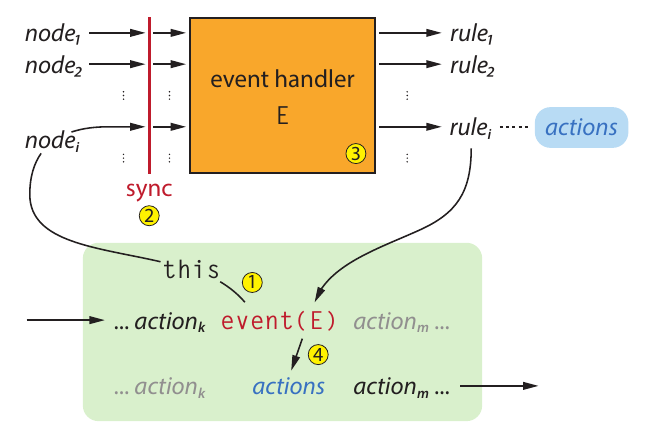
\includegraphics[width=11cm]{figuras/event_handler.png}
	}
	{\Fonte{\cite{schwarz2015}}}
\end{figure}

\newpage

\subsection{Linguagem}
\label{sec:linguagem_cga++}

Os recursos da \textit{CGA++} apresentados por \citeonline{schwarz2015} ainda são complementados por outros novos componentes de linguagem, que oferecem uma notação mais simples, aumentando a expressividade, conforme mostrados a seguir:

\textbf{Objetos suportados:} Além de tipos \textit{booleanos}, números e \textit{strings}, a \textit{CGA++} oferece suporte à listas e tuplas. As listas são sequências com um número arbitrário de valores do mesmo tipo. As tuplas representam sequências com um tamanho fixo de valores, podendo ser de tipos distintos. Além disso, a \textit{CGA++} também suporta funções anônimas, como o construto $[param_0, ...](body)$, que produz um novo valor de função, onde qualquer variável fora da função referenciada na expressão \textit{body} tem seu valor capturado como parte do valor da função.

\textbf{Argumentos de expressão:} Os argumentos de expressão visam facilitar a expressão e fornecer uma sintaxe sucinta, sendo suportados por muitas funções integradas que processam vários itens, como os elementos de uma lista.

\textbf{Argumentos iteráveis:} Se uma função receber uma lista como um argumento e avaliar um argumento de expressão para cada elemento desta lista, então, um nome significativo para acessar o respectivo elemento dentro do argumento de expressão pode ser especificado como parte do argumento de lista $(name:list)$. Se omitido, o elemento está disponível por meio de uma variável implícita.

\textbf{Operador de cadeia:} Ao aplicar, iterativamente, uma sequência de funções a um valor, o operador de cadeia \texttt{->} pode ser útil para melhorar a legibilidade, pois aplica seu lado esquerdo como primeiro argumento ao seu lado direito. Por exemplo,

\vspace{0.5cm}

\begin{description}
    \item[] \qquad \qquad $\texttt{this -> t(2, 0, 2) -> s(2, 9, 6) -> r(30, 0, 0)}$,
\end{description}

\vspace{0.5cm}

\noindent é equivalente a

\vspace{0.5cm}

\begin{description}
    \item[] \qquad \qquad $\texttt{r(s(t(this, 2, 0, 2), 2, 9, 6), 30, 0, 0)}$.
\end{description}

\vspace{0.5cm}

\textbf{Argumentos implícitos:} Em alguns cenários, existe um valor bem definido $\nu \in \mathbb{N}$, no qual, geralmente, uma função é aplicada. Visando a concisão notacional é possível, simplesmente, omitir esse valor. Por exemplo, se uma função interna aparecer dentro de um corpo de regra e aceitar uma forma como primeiro argumento, a forma atual (\texttt{this}) será usada automaticamente se este argumento for omitido. Da mesma maneira, a lista de formas participantes (\texttt{\$nodes}) é usada implicitamente como primeiro argumento em uma expressão do manipulador de evento.

\textbf{Variáveis auxiliares:} Ao lidar com expressões complexas ou usar o resultado de uma expressão diversas vezes, clareza e facilidade de formulação podem se beneficiar da introdução de variáveis para os valores de algumas expressões envolvidas. Para este fim, o novo construto

\vspace{0.5cm}

\begin{description}
    \item[] \qquad \qquad $\texttt{with}(var_1 = value_1, ..., expression)$
    \item[] \qquad \qquad $\texttt{with}(var_1 = value_1, ...) \{actions\}$
\end{description}

\vspace{0.5cm}

\noindent é fornecido, permitindo atribuir valores às variáveis e, posteriormente, usá-los em uma expressão ou dentro dos argumentos de ações.

Mais informações sobre a \textit{CGA++} foram disponibilizadas por \citeonline{schwarz2015} como material suplementar.

\subsection{Aplicações}
\label{sec:aplicacoes_cga++}

Com intuito de demonstrar os recursos de modelagem oferecidos pela \textit{CGA++}, \citeonline{schwarz2015} apresentam os seguintes exemplos, cobrindo diferentes domínios de aplicação:

\textbf{Planejamento urbano:} Uma tarefa comum dos planejadores urbanos é projetar o chamado bloco perimetral, ou seja, um lote de blocos com edifícios em seus limites, conforme mostrado na Figura \ref{fig:cga++_planejamento_urbano}.

\begin{figure}[h!]
	\centering
	\captionsetup{width=15cm}
	\Caption{\label{fig:cga++_planejamento_urbano} Representação de bloco perimetral. Acima: estratégia de modelagem desejada e os parâmetros envolvidos. Meio: exemplos de resultados para diferentes escolhas de parâmetros. Abaixo: exemplo de um resultado de planejamento urbano no mundo real.}	
	\UFCfig{}{
		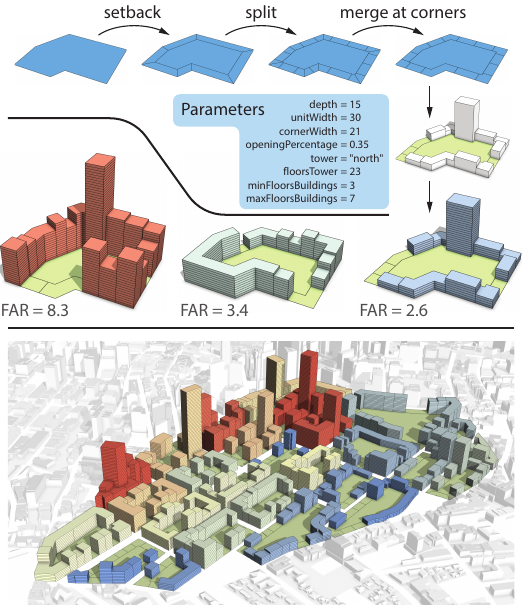
\includegraphics[width=15cm]{figuras/cga++_planejamento_urbano.png}
	}
	{\Fonte{\cite{schwarz2015}}}
\end{figure}

\newpage

\textbf{Edifícios:} Inspirados nos arranha-céus ecológicos de megacidades asiáticas, os modelos da Figura \ref{fig:cga++_buildings} consistem em, no máximo, dois blocos de torres, possuindo pisos deslocados e terraços com jardins no telhado, que são ligados por uma série de pontes suspensas.

\begin{figure}[h!]
	\centering
	\captionsetup{width=15cm}
	\Caption{\label{fig:cga++_buildings} Modelos de arranha-céus ecológicos. Acima: principais etapas da abordagem de modelagem. Abaixo: visualizações em foco do resultado do exemplo e resultados para diferentes valores para área com gramado.}	
	\UFCfig{}{
		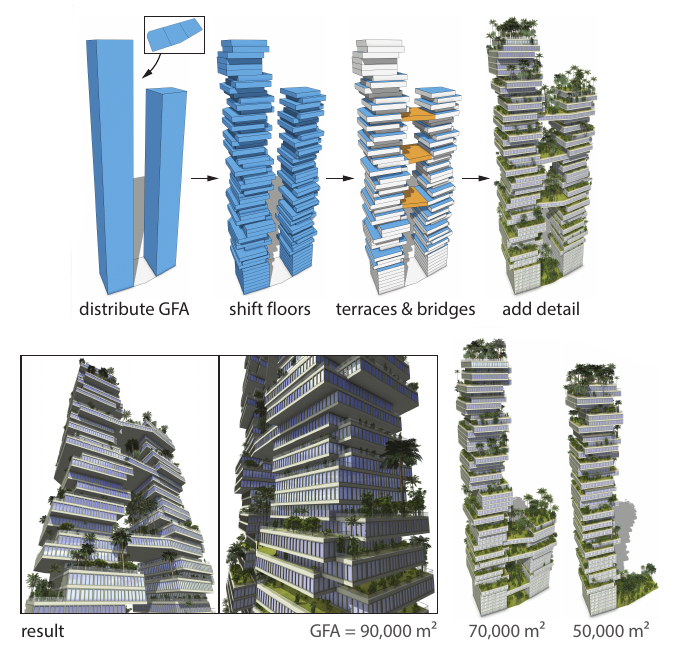
\includegraphics[width=15cm]{figuras/cga++_buildings_001.png}
	}
	{\Fonte{Adaptado de \cite{schwarz2015}}}
\end{figure}

\newpage

\textbf{Fachadas:} Na geração de fachadas aleatórias, o alinhamento desempenha um papel fundamental, assim, a Figura \ref{fig:cga++_fachadas} apresenta os recursos da \textit{CGA++} neste contexto.

\begin{figure}[h!]
	\centering
	\captionsetup{width=14cm}
	\Caption{\label{fig:cga++_fachadas} Modelos de fachadas com elementos e alinhamentos aleatórios. Acima: Abordagem de solução geral (as linhas de divisão são mostradas em vermelho). Abaixo: Exemplo de resultados para diferentes sementes aleatórias.}
	\UFCfig{}{
		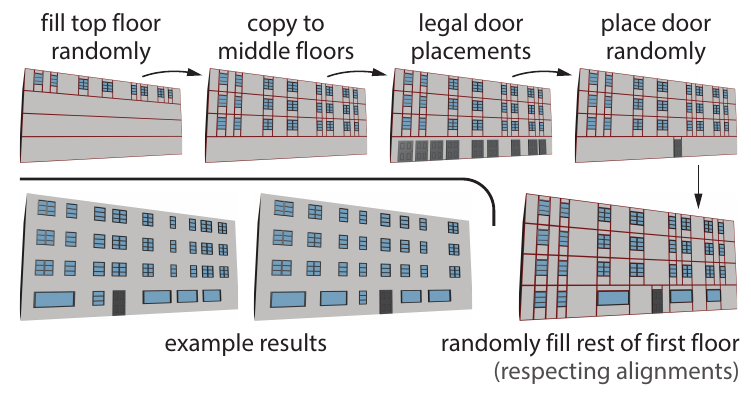
\includegraphics[width=13cm]{figuras/cga++_fachadas.png}
	}
	{\Fonte{\cite{schwarz2015}}}
\end{figure}

\newpage

\section{Selection Expressions}
\label{sec:selex}

A \gls{SELEX} é uma nova abordagem para geração procedural, que foi introduzida por \citeonline{wonka2018}, e tem como ideia principal selecionar formas utilizando \textit{selection-expressions}, no lugar da simples correspondência de \textit{strings} usada nas gramáticas atuais, como \textit{CGA Shape} e \textit{CGA++}. 

Segundo \citeonline{wonka2018}, uma \textit{selection-expression} especifica como selecionar um subconjunto complexo de formas em uma hierarquia de formas, por exemplo, "selecionar todas as janelas altas no segundo andar da fachada principal do edifício", o que permite expressar ideias de modelagem em seu contexto global, substituindo regras tradicionais que operam apenas localmente. Outro recurso da \gls{SELEX} é a aplicação de restrições de alinhamento e restrições de mesmo tamanho, permitindo que descrições procedurais possam gerar variações de fachadas e construções, sem violar as restrições de alinhamento e dimensionamento que afetam o estado da arte atual.

\citeonline{wonka2018} argumenta que o principal intuito de uma gramática é derivar um \textit{design} baseando-se em operações de divisão. Por exemplo, inicialmente, um modelo de massa é gerado. Após, as faces laterais do modelo de massa são extraídas como polígonos de fachada. Em seguida, os polígonos de fachada podem ser divididos em colunas ou pisos. Depois disso, os pisos podem ser divididos em ladrilhos e, por fim, em paredes, janelas ou portas. Desta maneira, a \gls{SELEX} visa melhorar dois problemas predominantes nesta abordagem.

Em primeiro lugar, \citeonline{wonka2018} afirma que a \textit{CGA Shape} fornece oportunidades limitadas para coordenar os diferentes ramos da derivação. Por exemplo, uma regra pode ser invocada para um ladrilho em algum lugar de um edifício para colocar uma janela e uma varanda. Depois, esta regra precisa decidir localmente como a janela e a varanda devem ser projetadas, de modo que as decisões de \textit{design} sejam coordenadas com todos os outros elementos de um edifício. Uma vez que o alinhamento correto dos elementos é difícil de modelar, a solução proposta é a introdução de construções de linguagem que possibilitam uma melhor comunicação entre as diferentes partes de um \textit{design}. A ideia principal é utilizar uma visão global para descrever as principais decisões de \textit{design} envolvidas na modelagem. Por exemplo, ao invés das janelas decidirem localmente que tamanho, alinhamento e tipo devem ter, são escritas regras globais que descrevam onde colocar quais tipos de janelas. Assim, há uma alteração das regras no formato $label \rightarrow actions$ para regras no formato $selection\mbox{-}expression \rightarrow actions$. Enquanto trabalhos anteriores se concentravam, principalmente, em melhorias no lado direito de uma regra, a \gls{SELEX} propõe extensões também no lado esquerdo de uma regra.

Em segundo lugar, \citeonline{wonka2018} afirma que existem algumas desvantagens na abordagem de divisão hierárquica utilizada pela \textit{CGA Shape} e \textit{CGA++}. Por exemplo, existem diversas maneiras de ver o mesmo edifício, ou seja, olhando para uma fachada, pode-se estar interessado em expressar uma operação de modelagem em termos de pisos, em termos de colunas ou um subconjunto de ladrilhos. Neste contexto, a escrita da regra força um edifício a ser dividido em uma única hierarquia, o que é um problema. Assim, se o autor da regra se comprometer com uma subdivisão com base no andar, será muito difícil expressar as operações de modelagem que precisam ser coordenadas entre várias colunas e vice-versa. Além disso, uma única hierarquia pode levar à uma quantidade desnecessária de regras e à regras que não têm semântica. Por exemplo, na Figura \ref{fig:cgaVSselex}(c), a fachada é dividida em uma região à esquerda, uma coluna da porta e uma região à direita. Em seguida, as regiões individuais são divididas em andares. Desta maneira, tal estrutura impõe uma hierarquia que tem regiões intermediárias desnecessárias que são difíceis de nomear semanticamente e apresentam problemas para formular seleções, por exemplo, todas as regiões coloridas na Figura \ref{fig:cgaVSselex}(c). Para superar essas limitações, a \gls{SELEX} permite o gerenciamento de várias hierarquias simultaneamente, oferecendo suporte à múltiplas visualizações dos dados sem dividir as formas.

 Na Figura \ref{fig:cgaVSselex}, \citeonline{wonka2018} ilustra os problemas com a abordagem anterior e as vantagens do uso da \gls{SELEX} em um exemplo selecionado: 
 
 \begin{description}
     \item[] \; (a) Fachada vazia;
     
     \item[] \; (b) Grades são usadas para permitir diferentes visualizações dos dados, como linhas, colunas, subgrades ou células individuais da grade;
     
     \item[] \; (c) Problemas de divisão das abordagens atuais, as quais não permitem a fusão de células. Desta maneira, ao se realizar divisões para estabelecer regiões de múltiplas células, sequências complexas e difíceis divisões verticais e horizontais alternadas são necessárias, o que é difícil de gerenciar;
     
     \item[] \; (d) A \gls{SELEX} permite selecionar, arbitrariamente, sub-grades retangulares de uma grade, e posicionar elementos em relação à elas, permitindo a modelagem de uma forma natural e semanticamente significativa;
     
     \item[] \; (e) Na geração de fachadas de edifícios, os elementos são organizados de acordo com uma grade para simplificar o alinhamento, contudo, elementos únicos podem abranger várias células da grade ou ser colocados entre as células da grade. Em particular, incorporar elementos que abrangem duas células, cada uma delas contendo um outro elemento, como os ornamentos amarelos e azuis no último andar. Para isso, a \gls{SELEX} fornece suporte à seleções sobrepostas, onde pode ser necessário a seleção de uma única célula para colocar cada janela, e uma seleção de célula dupla para colocar ornamentos, por exemplo.
 \end{description}
 

\begin{figure}[h!]
	\centering
	\captionsetup{width=15cm}
	\Caption{\label{fig:cgaVSselex} Ilustração dos paradigmas de modelagem \gls{SELEX} e \textit{CGA Shape}.}
	\UFCfig{}{
		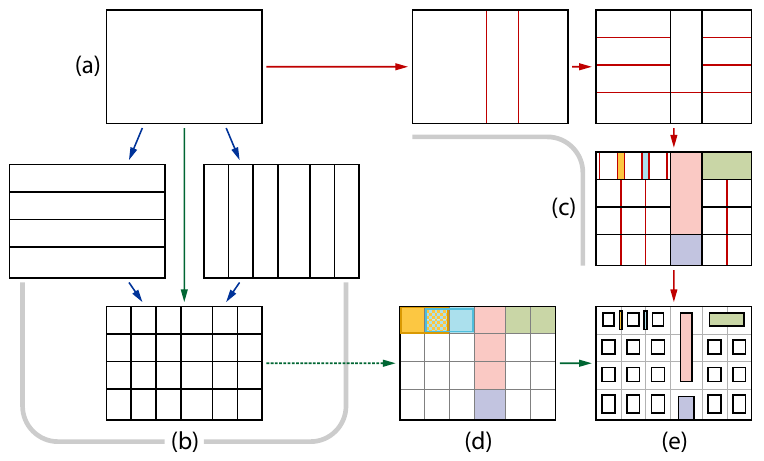
\includegraphics[width=14cm]{figuras/cgaVSselex.png}
	}
	{\Fonte{\cite{wonka2018}}}	
\end{figure}

\subsection{Definições de forma}
\label{sec:selex_definicao_formas}

\citeonline{wonka2018} argumenta que a \gls{SELEX} utiliza grades como formas virtuais, as quais são utilizadas para gerar qualquer sub-região como forma auxiliar, sem ter que gerar e gerenciar a sub-região explicitamente, conforme ilustrado na Figura \ref{fig:shapes_selex}(f). Existem, assim, dois tipos de formas diferentes: formas virtuais e formas de construção, onde, todas as outras formas que não são formas virtuais são chamadas formas de construção. As formas virtuais podem ser colocadas em uma forma de construção 2D. Normalmente, as formas virtuais possuem várias linhas e colunas, desse modo, consistem em múltiplas células. As formas virtuais orientam a colocação de outras formas de construção, mas não são usadas para dividir formas de construção. Para uma forma de construção, podem existir diversas formas virtuais, permitindo a modelagem de \textit{layouts} complexos. 

Conforme apresentado por \citeonline{wonka2018}, formas virtuais podem ser utilizadas nos seguintes casos:

\begin{itemize}
    \item Alocar uma posição a partir da seleção de uma célula da grade, na qual determinada forma pode ser adicionada;
    
    \item Facilitar a seleção das formas de construção que estão contidas dentro delas, por exemplo, para selecionar formas na mesma linha ou coluna;
    
    \item Definir o comportamento de redimensionamento, uma vez que a especificação da grade inclui informações sobre o espaçamento de linhas e colunas, e a forma como as linhas e colunas se repetem se houver espaço  disponível.
\end{itemize}

\begin{figure}[h!]
	\centering
	\captionsetup{width=15cm}
	\Caption{\label{fig:shapes_selex} Diferentes opções de \textit{design} com \gls{SELEX}.}
	\UFCfig{}{
		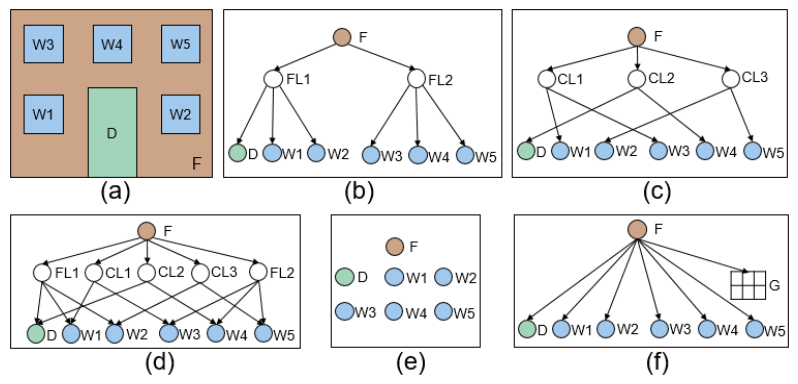
\includegraphics[width=15cm]{figuras/shapes_selex.png}
	}
	{\Fonte{\cite{wonka2018}}}	
\end{figure}

De acordo com \citeonline{wonka2018}, a \gls{SELEX} utiliza um conjunto de atributos integrados para cada forma. \textit{Label} é o nome da forma, por exemplo, \textit{"window"}, podendo ser único ou compartilhado entre várias formas. O \textit{Type} indica se a forma é uma forma virtual (\textit{"virtual"}), uma forma de construção (\textit{"construction"}) ou uma célula (\textit{"cell"}) de uma forma virtual. \textit{Dim} é uma variável binária que indica uma forma 2D ou 3D. O escopo descreve uma caixa orientada no espaço 3D, utilizando variáveis que descrevem um quadro de coordenadas $(xaxis, yaxis, zaxis)$, uma posição em $R^3$ (denotada por $xpos$, $ypos$, $zpos$) e informações de tamanho \textit{(xsize, ysize, zsize)}.

\citeonline{wonka2018} afirma que a linguagem da \gls{SELEX} desenvolve uma hierarquia de formas e as armazena em uma árvore, por meio da utilização de certas funções. Cada forma pode ter apenas um pai, e apenas formas de construção podem ter filhos. As formas não podem ser excluídas, mas podem ser definidas como invisíveis. O nó raiz é uma forma com o rótulo \textit{"root"}. As formas 2D são utilizadas para criar subdivisões em outras formas 2D, por exemplo, fachadas ou janelas. As formas 3D são utilizadas para modelar elementos que são extrudados da fachada ou estruturas suspensas, por exemplo, uma varanda ou um ornamento na janela. Na hierarquia de formas da \gls{SELEX}, as formas têm filhos que são formas anexadas ou formas contidas. Uma forma anexada é uma forma 3D vinculada à uma forma 2D. Em algumas situações, a forma anexada tem uma face contida na forma 2D, às vezes, as formas não se tocam. Como exemplo, a forma 3D de uma varanda pode ser anexada à uma forma 2D, que descreve a posição da janela dentro de uma fachada. Uma forma contida é uma forma 2D contida dentro de sua forma 2D pai, ou uma face lateral de uma forma 3D pai. Uma forma conectada é uma forma 2D que compartilha uma aresta com outra forma 2D. Topologicamente, uma forma conectada é considerada uma vizinha no contexto de \textit{selection-expressions}. A Figura \ref{fig:shapes3D_selex} ilustra o conceito de formas conectadas e formas contidas.

\begin{figure}[h!]
	\centering
	\captionsetup{width=15cm}
	\Caption{\label{fig:shapes3D_selex} Para a forma atual (\textit{leftWall}), é demonstrada uma forma contida (\textit{win}), uma forma anexada (\textit{balcony}) e uma forma conectada (\textit{cornerWall}).}
	\UFCfig{}{
		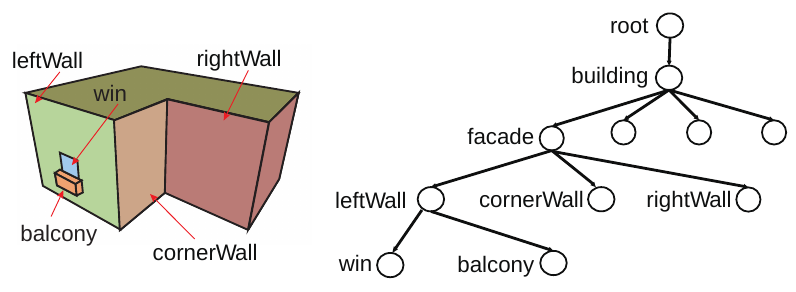
\includegraphics[width=15cm]{figuras/shapes3D_selex.png}
	}
	{\Fonte{\cite{wonka2018}}}	
\end{figure}

\newpage

\subsection{Introdução à linguagem}
\label{sec:introducao_selex}

\citeonline{wonka2018} explica que a linguagem de modelagem procedural \gls{SELEX} executa um comando por vez, podendo ser uma regra ou uma atribuição de variável. Uma regra tem o seguinte formato:

\vspace{0.5cm}

\begin{description}
    \item[] \qquad \qquad $selection\mbox{-}expression \rightarrow actions$,
\end{description}

\vspace{0.5cm}

\noindent na qual a \textit{selection-expression} seleciona uma lista de formas da árvore de formas atual, e as \textit{actions} são comandos executados em cada forma na lista. Por exemplo, na Figura \ref{fig:code_selex}, os comandos de C2 a C11 são regras. Uma atribuição tem o formato:

\vspace{0.5cm}

\begin{description}
    \item[] \qquad \qquad $identifier = expression$,
\end{description}

\vspace{0.5cm}

\noindent na qual o \textit{identifier} denota uma variável e a \textit{expression} avalia um valor. Por exemplo, na Figura \ref{fig:code_selex}, os comandos rotulados como $C1$ são atribuições de variáveis. Uma lista é uma lista de outros tipos de objetos, mas também há suporte para listas de listas. Um par consiste em dois objetos, no qual o primeiro objeto deve ser comparável, podendo ser um número, uma \textit{string} ou um valor \textit{booleano}, e o segundo objeto pode ser qualquer tipo de objeto. Além disso, a linguagem também oferece suporte à construções de linguagem comuns, como seleção aleatória e condicionais.

\begin{figure}[h!]
	\centering
	\captionsetup{width=15cm}
	\Caption{\label{fig:code_selex} Instruções \gls{SELEX} para gerar a Figura \ref{fig:cgaVSselex}(e).}
	\UFCfig{}{
		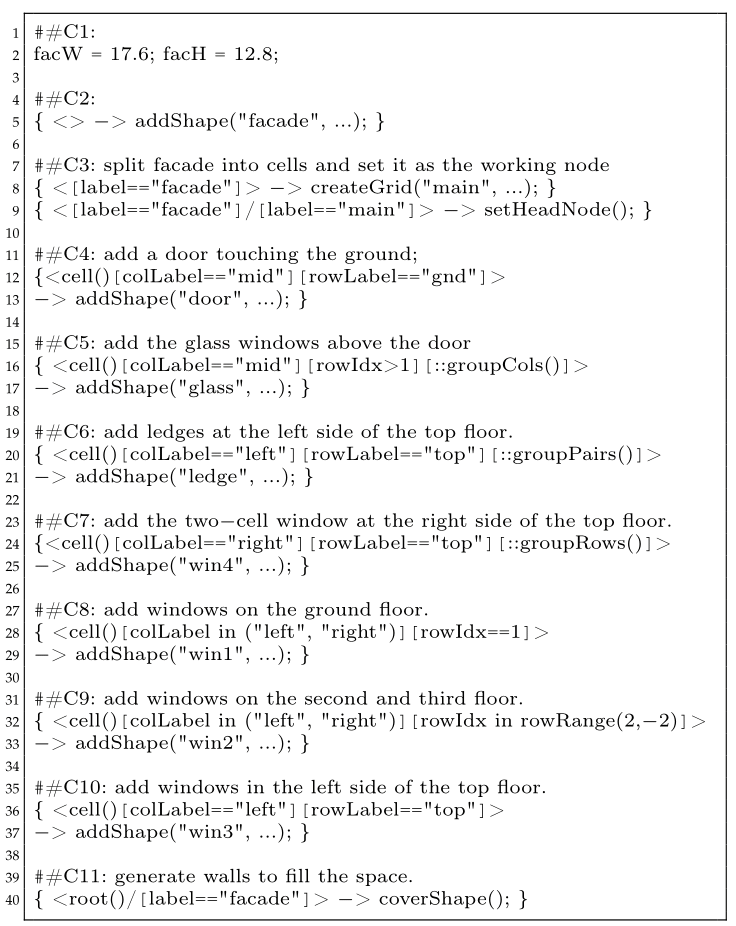
\includegraphics[width=15cm]{figuras/code_selex.png}
	}
	{\Fonte{\cite{wonka2018}}}	
\end{figure}

\newpage

\subsection{Modelagem procedural baseada em seleção}
\label{sec:modelagem_selecao}

Segundo \citeonline{wonka2018}, o recurso mais importante da \gls{SELEX} são as \textit{selection-expressions}, que permitem selecionar uma lista de formas de uma árvore de formas utilizando seletores intercalados com o operador "$/$". Cada seletor recebe uma lista de formas como entrada e retorna uma lista de formas. A entrada implícita para o primeiro seletor é uma lista contendo o nó raiz da árvore de formas. O operador "$/$" \, obtém uma lista de formas como entrada e executa os comandos restantes para cada forma na lista. 

\citeonline{wonka2018} argumenta que seletores são agrupados em sequências de seletores especializados, podendo ser de três tipos diferentes: seletor de topologia, por exemplo, "\textit{child}", "\textit{descendant}"; seletor de atributo, por exemplo, "$[label=="window"]$"; e seletor de grupo, por exemplo "$[::groupRows()]$". Os seletores precisam ocorrer na ordem em que foram fornecidos, não podendo ser misturados em uma sequência arbitrária. 

Na definição de \citeonline{wonka2018}, uma \textit{selection-expression} possui a seguinte configuração:

\vspace{0.5cm}

\begin{description}
    \item[] \qquad \qquad $<[topoS] [attrS | groupS]^* / [topoS] [attrS | groupS]^* / ... >$,
\end{description}

\vspace{0.5cm}

\noindent onde, dentro de cada sequência de seletor, há de zero a um seletores de topologia (\textit{topoS}), zero a muitos seletores de atributo (\textit{attrS}), e zero a muitos seletores de grupo (\textit{groupS}). Uma \textit{selection-expression} vazia retorna a entrada. Quando uma forma que não existe é especificada, a seleção correspondente retornará uma forma vazia e a regra não será executada. Um exemplo é mostrado na Figura \ref{fig:graph_selex}, por meio de um grafo abstrato, no qual os nós selecionados pela \textit{selection-expression} 

\vspace{0.5cm}

\begin{description}
    \item[] \qquad \qquad $<[label="A"] / [label="C"] [h \geq 2]>$
\end{description}

\vspace{0.5cm}

\noindent são destacados em verde. No processo, a \textit{selection-expression} seleciona os filhos rotulados como "$A$" \, do nó raiz, então, para os dois nós rotulados como "$A$", todos os seus filhos rotulados como "$C$", \, com um valor de atributo $h \geq 2$, são selecionados.

\begin{figure}[h!]
	\centering
	\captionsetup{width=15cm}
	\Caption{\label{fig:graph_selex} Grafo abstrato da seleção de nós.}
	\UFCfig{}{
		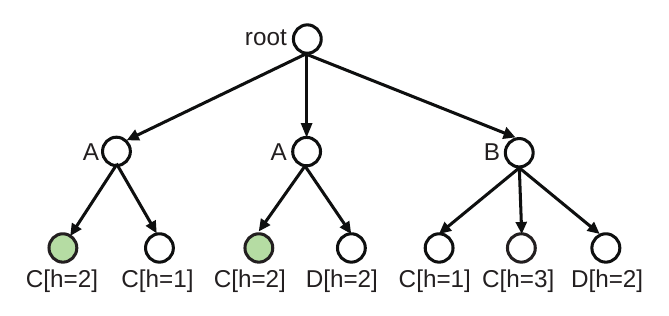
\includegraphics[width=13cm]{figuras/graph_selex.png}
	}
	{\Fonte{\cite{wonka2018}}}	
\end{figure}

Por se tratar de um importante recurso da \gls{SELEX}, \citeonline{wonka2018} apresenta algumas especificações mais detalhadas sobre os diferentes tipos de seletores:

\textbf{Seletor de topologia:} Recebe uma lista contendo uma única forma como entrada, e produz uma lista de formas com a relação de topologia especificada para a forma de entrada. Um seletor de topologia tem a forma $[topology\mbox{-}function()]$, e pode utilizar uma das seguintes funções: "$child()$", "$descendant()$", "$parent()$", "$root()$", "$neighbor()$", e "$contained()$". A função "$contained()$" \, é o padrão para uma forma virtual e "$child()$" \, é o padrão para uma forma de construção.

\textbf{Seletor de atributo:} A entrada é uma lista de formas e retorna uma lista de formas cujos atributos satisfazem algumas condições. Em sua estrutura básica, um seletor de atributo tem a configuração $[attributename \;\; comparison \:\; value]$. O operador de comparação é especificado como em outras linguagens de programação, por exemplo, $==$, $<=$, $>=$, $!=$ e "$in$". Os exemplos são "$[label="facade"]$" \, e "$[label \, in \, ("window\_arch", "window\_rect")]$". Alternativamente, em sua estrutura mais geral, um seletor de atributo é uma expressão booleana. Os exemplos são "$[isEmpty()]$", "$[numCols()>4]$" \, ou "$[toShapeX(0.5)>2]$". A função "$toShapeX(0.5)$" \, dimensiona o valor de entrada $0.5$ pelo "\textit{xsize}" \, de uma forma. Uma função importante é "$pattern(regex, pat)$", que verifica se o padrão de caracteres de "\textit{regex}", na posição do índice de uma forma, corresponde à "\textit{pat}". Por exemplo, "$pattern("(AB)^*","A")$" \, testa se uma forma de entrada está em uma posição de índice ímpar, e "$pattern("A(B)^*A","A")$" \, testa se uma forma de entrada está na primeira ou na última posição de uma lista de entrada. As funções "$isEven()$" \, e "$isOdd()$" \, são casos especiais do comando "$pattern(regex, pat)$", que verificam se uma forma tem um índice par ou ímpar em uma lista de formas selecionadas. Os atributos "\textit{rowIdx}" \, e "\textit{colIdx}" \, são utilizados como a posição topológica de uma célula em relação à região abrangida pelas formas virtuais de entrada. Por exemplo, "$rowIdx==1 \, \&\& \, colIdx==1$" \, especifica a célula inferior superior de uma grade. 

\textbf{Seletor de grupo:} Recebe uma lista de formas como entrada e aplica operações de agrupamento para retornar uma lista de formas combinadas. Um seletor de grupo opera apenas em formas virtuais e reagrupa sub-regiões, por exemplo, combinando células de uma forma virtual em pisos. Os seletores de grupo são implementados usando funções de agrupamento, resultando em seletores na seguinte configuração: $[::grouping\mbox{-}function()]$. Algumas funções que operam juntamente com seletores de grupo são:

\begin{itemize}
    \item $groupRows()$ \, e $groupCols()$: mesclam formas virtuais adjacentes, ou seja, \textit{cells}, com o mesmo índice de linha ou coluna;
    
    \item $groupRegions()$: mescla todas as formas virtuais adjacentes que formam uma ou várias regiões retangulares;
    
    \item $groupEach(n)$: mescla todas as $n$ formas virtuais adjacentes.
    
    \item $groupPair()$: gera todos os pares possíveis de duas formas subsequentes. Por exemplo, dado "$ABCD$", ele retornará "$AB$", "$BC$" \, e "$CD$";
    
    \item $cells()$: decompõe uma forma virtual como uma lista de formas virtuais com uma célula;
    
    \item $sortBy(d, pos, order=1)$: classifica as formas selecionadas pela posição relativa "\textit{pos}", na dimensão "$d$", na ordem crescente ($order=1$) ou decrescente ($order=0$).
\end{itemize}

\vspace{0.5cm}

Na Figura \ref{fig:seletores}, \citeonline{wonka2018} ilustra a utilização de alguns seletores:

\vspace{0.5cm}

\begin{description}
    \item[] \; (a) Uma grade é utilizada para demonstrar múltiplas seleções
    \item[] \; (b) $<descendant()[label=="facade"]/[label=="mainGrid"]/[type=="cell"]$ \\
    \qquad \qquad \qquad $[rowIdx \, in \, (1,2)][colIdx==3]>$ 
    \item[] \; (c) $<descendant()[label=="facade"]/[label=="mainGrid"]/[type=="cell"]$ \\
    \qquad \qquad \qquad $[rowIdx \, in \, (3,4)][colIdx \, in \, (1,2,4,5)][::groupRegions()]>$
    \item[] \; (d) $<descendant()[label=="facade"]/[label=="mainGrid"]/[type=="cell"]$ \\
    \qquad \qquad \qquad $[rowIdx \, in \, (1,2)][colIdx \, in \, (2,4)][::group\mbox{-}Cols()][::cells()]>$
    \item[] \; (e) Representação da árvore de formas
\end{description}

\vspace{0.5cm}

\begin{figure}[h!]
	\centering
	\captionsetup{width=15cm}
	\Caption{\label{fig:seletores} Exemplo da utilização de seletores.}
	\UFCfig{}{
		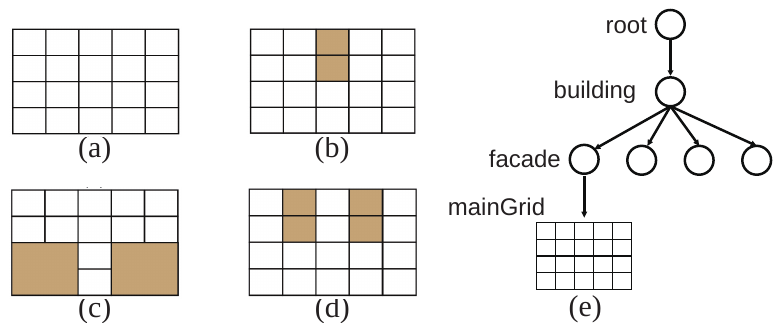
\includegraphics[width=13cm]{figuras/seletores.png}
	}
	{\Fonte{\cite{wonka2018}}}	
\end{figure}

\subsection{Ações}
\label{sec:selex_acoes}

As ações são descritas por \citeonline{wonka2018} como uma sequência de funções, que podem ser executadas para cada forma na lista de formas, gerada por uma \textit{selection-expression}.

\citeonline{wonka2018} afirma que as ações mais importantes são funções usadas para criar novas formas, por exemplo, "\textit{addShape}", "\textit{attachShape}", "\textit{coverShape}" \, e "\textit{connectShape}", que criam novas formas e as adicionam na hierarquia de formas atual. O pai de uma nova forma pode ser especificado explicitamente ou implicitamente usando valores padrão. Normalmente, o pai é a forma de construção de entrada ou, no caso de uma forma virtual, o primeiro ancestral que é uma forma de construção. A Figura \ref{fig:acoes_selex}(a) mostra um exemplo da função "\textit{addShape}". Para gerar a fachada da Figura \ref{fig:cgaVSselex}. As instruções da Figura \ref{fig:code_selex} fazem uso intensivo da função "\textit{addShape}", uma vez que o exemplo é 2D.

Conforme argumentado por \citeonline{wonka2018}, outro aspecto da modelagem de edifícios residenciais complexos é que eles exigem um controle cuidadoso sobre a geometria que está sendo gerada. Para isso, são utilizados comandos para criar geometria dentro de formas que não são cobertas por outras formas com a função "\textit{coverShape}", como na Figura \ref{fig:acoes_selex}(b). Além disso, a \gls{SELEX} também fornece diversas funções para criar formas virtuais (grades), como no exemplo da Figura \ref{fig:acoes_selex}(c).

\begin{figure}[h!]
	\centering
	\captionsetup{width=15cm}
	\Caption{\label{fig:acoes_selex} Exemplo da utilização de ações.}
	\UFCfig{}{
		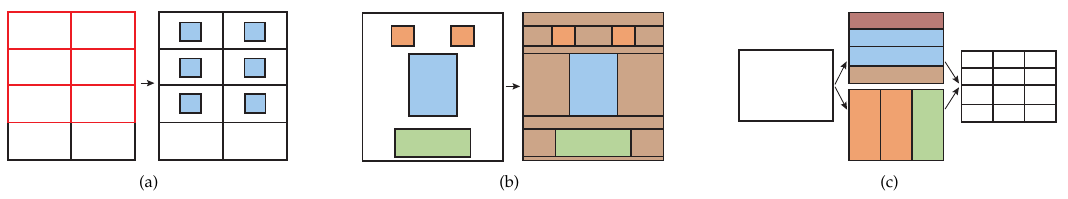
\includegraphics[width=15cm]{figuras/acoes_selex.png}
	}
	{\Fonte{\cite{wonka2018}}}	
\end{figure}

\subsection{Funções de restrição}
\label{sec:selex_funcoes}

Segundo \citeonline{wonka2018}, é difícil especificar a localização de uma forma em uma gramática estocástica, pois não é possível saber exatamente quais formas foram colocadas anteriormente e onde estão. Neste contexto, a \gls{SELEX} permite que seja definida uma sequência de restrições a partir do seguinte comando:

\vspace{0.5cm}

\begin{description}
    \item[] \qquad \qquad $constrain(constraint1, constraint2, ...)$.
\end{description}

\vspace{0.5cm}

Em seguida, as restrições especificadas são traduzidas em restrições lineares de uma formulação de programação quadrática inteira mista. As restrições lineares suportadas pela \gls{SELEX} são de alinhamento, simetria, distância até a borda e prevenção de interseção.

\citeonline{wonka2018} considera duas opções de \textit{design} para o problema de alinhamento. A primeira escolha de \textit{design} é decidir se as linhas de ajuste devem ser colocadas explicitamente por um comando, ou ser definidas implicitamente pelos limites das formas geradas numa etapa anterior. A segunda opção de \textit{design} é decidir se as linhas de ajuste devem ser nomeadas com um rótulo ou não. Na Figura \ref{fig:restricao_selex1}, é mostrado um exemplo comparando o ajuste com e sem rótulos, no qual: 

\begin{description}
    \item[] \; (a) Dado um \textit{layout} inicial com as formas $a$, $b$ e $c$;
    
    \item[] \; (b) Uma nova forma rotulada $d$ é adicionada;
    
    \item[] \; (c) No ajuste sem rótulos, a forma $d$ se encaixa nas linhas de ajuste mais próximas, ou seja, à esquerda da forma $a$ e à esquerda da forma $c$;
    
    \item[] \; (d) Utilizar ajuste com rótulos permite um controle mais preciso, por exemplo, ajustando a coordenada x do centro da forma $d$ à coordenada x ao centro da forma $a$.
\end{description}

\begin{figure}[h!]
	\centering
	\captionsetup{width=15cm}
	\Caption{\label{fig:restricao_selex1} Comparação do ajuste com e sem o uso de rótulos.}
	\UFCfig{}{
		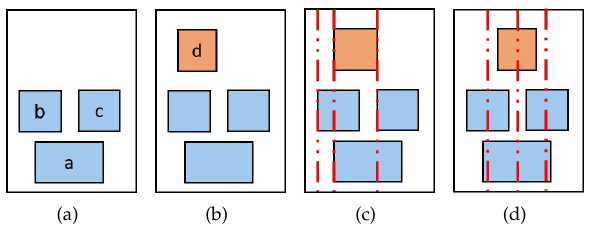
\includegraphics[width=15cm]{figuras/restricoes_selex1.png}
	}
	{\Fonte{\cite{wonka2018}}}	
\end{figure}

Conforme apresentado por \citeonline{wonka2018}, o alinhamento pode ser especificado de duas maneiras: uma forma de entrada e uma forma de referência especificada por um rótulo de forma. Os tipos de alinhamento suportados pela \gls{SELEX} são: "\textit{left}", "\textit{right}", "\textit{top}", "\textit{bottom}", "$center\mbox{-}x$", "$center\mbox{-}y$", "$one2two\mbox{-}x$", "$one2two\mbox{-}y$". Por exemplo, a função 

\vspace{0.5cm}

\begin{description}
    \item[] \qquad \qquad $constrain(snap2("window1", "left"), snap2("window1", "center\mbox{-}x"))$
\end{description}

\vspace{0.5cm}

\noindent especifica que uma forma de entrada deve ser alinhada à esquerda e ao centro x em relação à uma forma identificada como "\textit{window}". Os exemplos de "\textit{left}" \, e "$one2two\mbox{-}x$" \, são ilustrados na Figura \ref{fig:alinhamento_selex}, onde: (a) "\textit{left}" \, alinha a forma de entrada em verde à uma forma de referência em branco, e (b) "$one2two\mbox{-}x$" \, alinha a forma de entrada em verde ao centro da caixa delimitadora de duas formas de referência brancas. A linha tracejada vermelha indica a posição de ajuste, enquanto a caixa delimitadora vermelha marca a delimitação de duas formas de referência.

\begin{figure}[h!]
	\centering
	\captionsetup{width=15cm}
	\Caption{\label{fig:alinhamento_selex} Dois exemplos de alinhamento.}
	\UFCfig{}{
		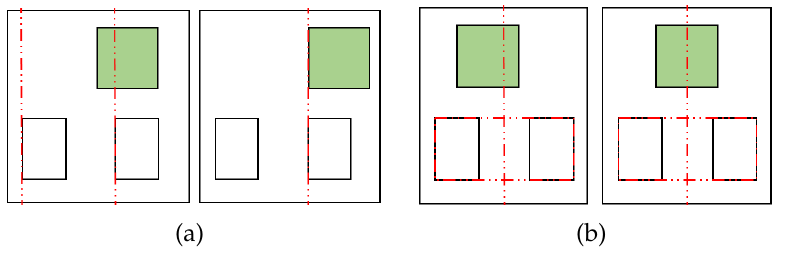
\includegraphics[width=15cm]{figuras/selex_alinhamento.png}
	}
	{\Fonte{\cite{wonka2018}}}	
\end{figure}

Especificações adicionais sobre a \gls{SELEX} foram disponibilizadas por \citeonline{wonka2018} como material suplementar.

\subsection{Aplicação}
\label{sec:selex_modelagem}

Na Figura \ref{fig:exemplo_selex}, \citeonline{wonka2018} ilustra a utilização de formas virtuais e \textit{selection-expressions} no processo de modelagem de um edifício, a partir das seguintes etapas:

\begin{description}
    \item[] \; (a) Polígono da planta especificada pelo usuário;
    
    \item[] \; (b) O polígono da planta é extrudado em um edifício;
    
    \item[] \; (c) Todas as fachadas do edifício são divididas em andares adicionando uma grade como uma forma virtual;
    
    \item[] \; (d) Cada fachada herda as informações do piso e é dividida em uma grade mais fina, especificando colunas, que são rotuladas com "\textit{colLeft}", "\textit{colMidLeft}", "\textit{colMidRight}" \, e "\textit{colRight}";
    
    \item[] \; (e) As colunas são selecionadas pelo rótulo "\textit{colMidLeft}";
    
    \item[] \; (f) As colunas são selecionadas pelo rótulo "\textit{colMidRight}" \, e a operação \textit{push} é aplicada na região rotulada com "\textit{colMidLeft}";
    
    \item[] \; (g) As colunas são selecionadas pelo rótulo "\textit{rowDown}" \,e a operação de \textit{pull} é aplicada nas regiões rotuladas com "\textit{colMidRight}" \, e "\textit{rowDown}", formando a massa do edifício;
    
    \item[] \; (h) Uma sub-região no lado esquerdo é selecionada e uma sub-grade é adicionada;
    
    \item[] \; (i) Conjuntos de células na grade principal são selecionadas para adicionar formas abrangendo várias células;
    
    \item[] \; (j) Linhas pares/ímpares em uma sub-região da segunda linha à última linha são selecionadas;
    
    \item[] \, (k) Uma forma de conexão é selecionada;
    
    \item[] \; (l) Linhas pares/ímpares são selecionadas e sub-grades diferentes são adicionadas;
    
    \item[] (m) Colunas largas e estreitas são selecionadas para adicionar janelas;
    
    \item[] \, (n) Janelas e portas extras são adicionadas;
    
    \item[] \, (o) Complementos são adicionados.
\end{description}

\begin{figure}[h!]
	\centering
	\captionsetup{width=15cm}
	\Caption{\label{fig:exemplo_selex} Exemplo de modelagem utilizando \gls{SELEX}.}
	\UFCfig{}{
		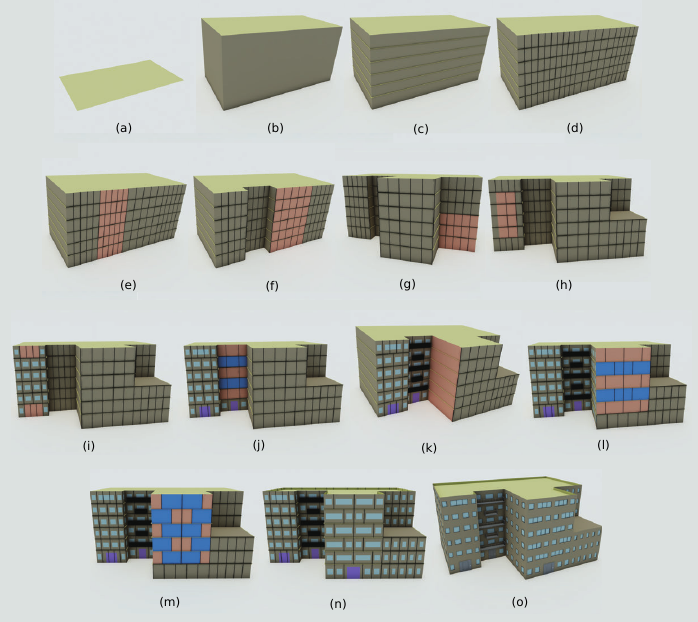
\includegraphics[width=15cm]{figuras/selex_exemplo_001.png}
	}
	{\Fonte{Adaptado de \cite{wonka2018}}}	
\end{figure}

\vspace{0.5cm}

\newpage

Uma vez que algumas das principais técnicas para geração procedural de edifícios foram apresentadas, na próxima seção, será abordado o conceito de deformação, bem como sua relação com a modelagem procedural.

\section{Deformação}
\label{sec:deformacao}

No campo da física, a deformação de uma estrutura é qualquer mudança da configuração geométrica do corpo que leve à uma variação da sua forma ou das suas dimensões, após a aplicação de uma ação externa \cite{truesdell1992}. Na área da Computação Gráfica, por sua vez, a modelagem de sólidos é uma das técnicas essenciais utilizadas em modeladores 3D comuns, como Maya, Rhinoceros e Blender, onde a modificação dos objetos é realizada, frequentemente, por meio da deformação de forma livre \cite{jana2017}.

Baseado neste contexto, a próxima seção é voltada para uma breve apresentação de algumas técnicas de deformação existentes. 

\subsection{Técnicas de deformação}
\label{sec:tecnicas_deformacao}

A deformação espacial é uma técnica importante no \textit{design} de formas. Idealizada por \citeonline{sedeberg1986}, a deformação de forma livre é uma transformação do espaço. Nela, é definida uma grade regular de pontos de controle, os quais podem ser descritos por uma combinação linear. Ao deslocar esses pontos de controle, uma deformação do espaço é alcançada. Geralmente, estes pontos de controle são espaçados regularmente na caixa delimitadora do elemento a ser deformado, conforme ilustrado na Figura \ref{fig:sedeberg}.

\begin{figure}[h!]
	\centering
	\captionsetup{width=15cm}
	\Caption{\label{fig:sedeberg} À esquerda, um exemplo de deformação livre dos objetos do cenário, a partir da mudança dos pontos da grade cúbica visível à direita.}
	\UFCfig{}{
		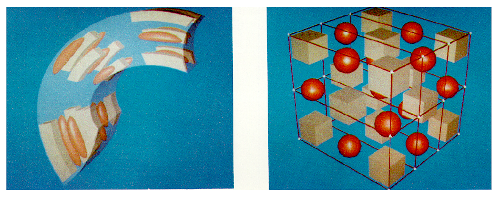
\includegraphics[width=13cm]{figuras/sedeberg.png}
	}
	{\Fonte{\cite{sedeberg1986}}}	
\end{figure}

Uma evolução do trabalho de \citeonline{sedeberg1986} é trazida por \citeonline{jin2000}, onde é apresentado um método de deformação tridimensional utilizando coordenadas polares direcionais. O usuário especifica um objeto de controle de origem e um objeto de controle de destino (Figura \ref{fig:jin_exemplo1}), que atuam como espaços de incorporação. Os objetos de controle de origem e de destino determinam uma transformação de volume tridimensional, que mapeia o espaço anexado no objeto de controle de origem para aquele do objeto de controle de destino (Figura \ref{fig:jin_exemplo2}). Ao incorporar o objeto a ser deformado no objeto de controle de origem, a transformação tridimensional do volume determina o objeto deformado automaticamente, sem o movimento dos pontos de controle.

\begin{figure}[h!]
	\centering
	\captionsetup{width=15cm}
	\Caption{\label{fig:jin_exemplo1} Objeto de controle de origem (a) e objetos de destino (b), (c), (d). $O_S$ e $O_D$ representam os respectivos centros dos objetos.}
	\UFCfig{}{
		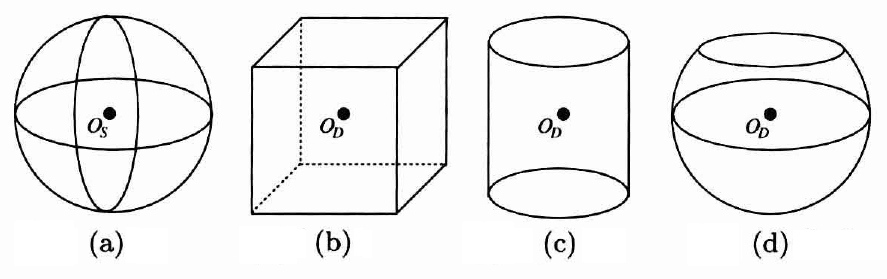
\includegraphics[width=14cm]{figuras/jin_exemplo1.png}
	}
	{\Fonte{Adaptado de \cite{jin2000}}}	
\end{figure}

\begin{figure}[h!]
	\centering
	\captionsetup{width=15cm}
	\Caption{\label{fig:jin_exemplo2} Deformação de uma bola de futebol com base nos objetos da Figura \ref{fig:jin_exemplo1}.}
	\UFCfig{}{
		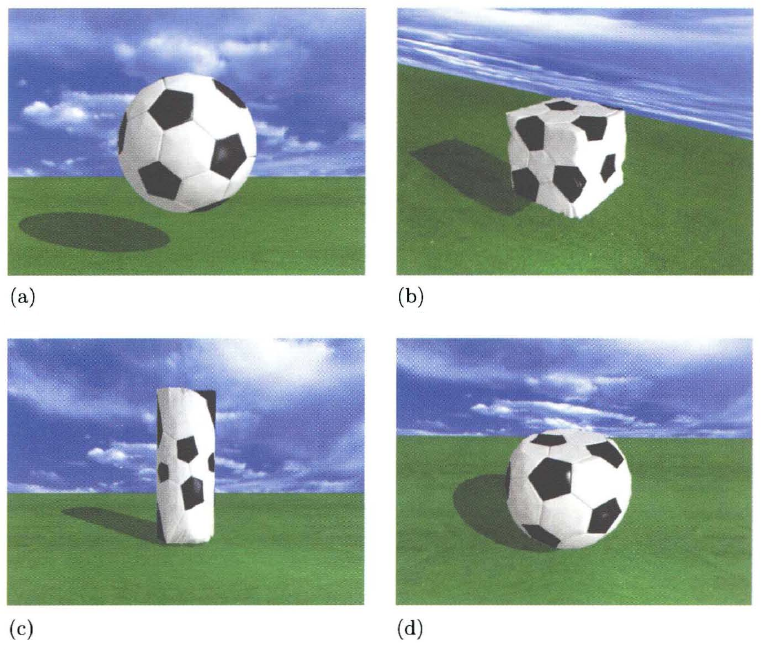
\includegraphics[width=10cm]{figuras/jin_exemplo2.png}
	}
	{\Fonte{Adaptado de \cite{jin2000}}}	
\end{figure}

Outras duas técnicas são apresentadas por \citeonline{jana2017}, o esquema de \citeonline{sedeberg1986} baseado em polinômios de Bernstein, que é a base das técnicas de deformação de forma livre (Figura \ref{fig:sedeberg_ffd}), e o método \gls{NURBS}, que utilizada um escopo mais elaborado e operações mais complexas (Figura \ref{fig:nurbs_ffd}).

\begin{figure}[h!]
	\centering
	\captionsetup{width=15cm}
	\Caption{\label{fig:sedeberg_ffd} Técnica de deformação de forma livre de Sederberg: a) antes e b) depois da transformação.}
	\UFCfig{}{
		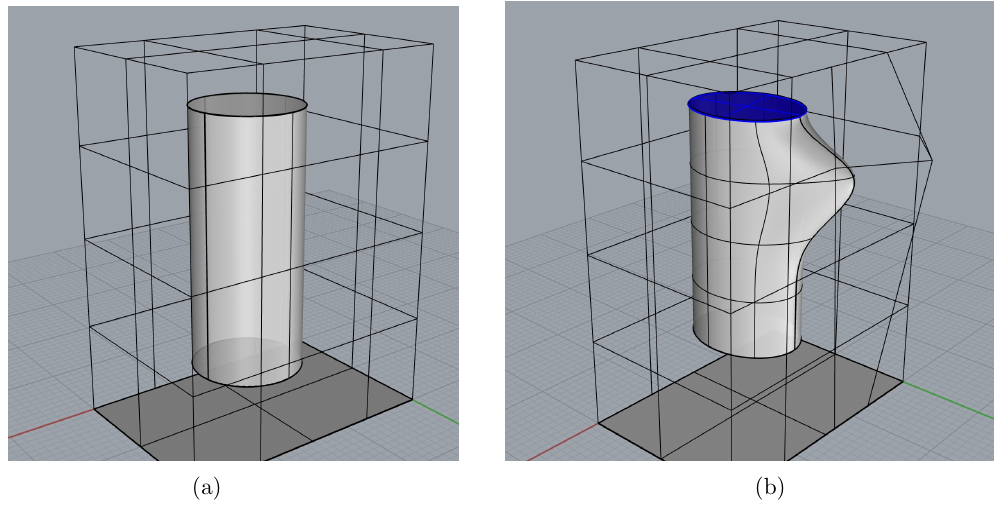
\includegraphics[width=13cm]{figuras/sedeberg_ffd.png}
	}
	{\Fonte{\cite{jana2017}}}	
\end{figure}

\begin{figure}[h!]
	\centering
	\captionsetup{width=15cm}
	\Caption{\label{fig:nurbs_ffd} Técnica de deformação de forma livre utilizando \gls{NURBS}: a) antes e b) depois da transformação.}
	\UFCfig{}{
		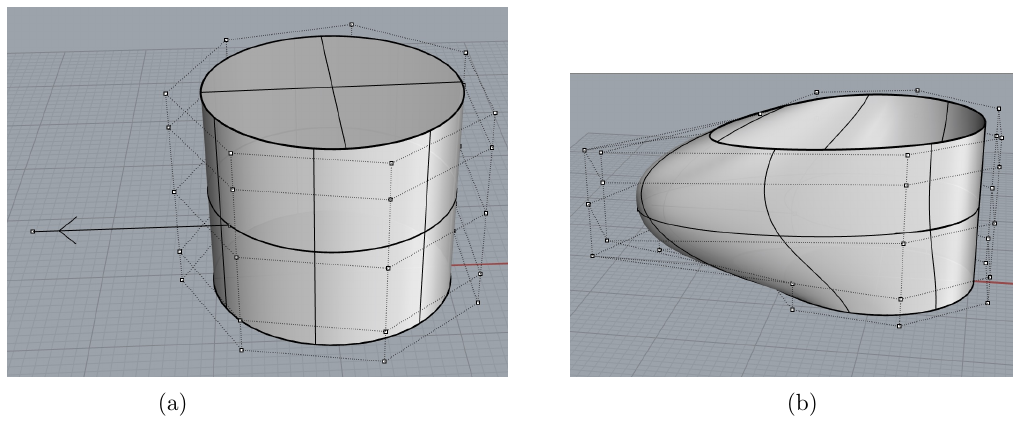
\includegraphics[width=13cm]{figuras/nurbs_ffd.png}
	}
	{\Fonte{\cite{jana2017}}}	
\end{figure}

Por achar o uso de caixas insatisfatório, \citeonline{fellner2013} argumenta que uma maior variedade de formas pode ser obtida pelo uso de poliedros convexos como delimitador de volumes, pois as operações de divisão não ficam mais limitadas aos três eixos principais, podendo-se utilizar planos arbitrários. Essas divisões permitem uma decomposição volumétrica em elementos convexos, uma vez que poliedros convexos podem representar diversas formas muito mais fielmente do que caixas. Um exemplo é mostrado na Figura \ref{fig:convex_example}, onde: (a) em um poliedro convexo, (b) um orifício circular é cortado deixando dois resultados, (c) uma parte interna convexa e (d) os arredores não convexos. A borda vermelha mostra o escopo convexo correspondente, que é igual ao escopo original.

\begin{figure}[h!]
	\centering
	\captionsetup{width=15cm}
	\Caption{\label{fig:convex_example} Uma operação de furo redondo.}
	\UFCfig{}{
		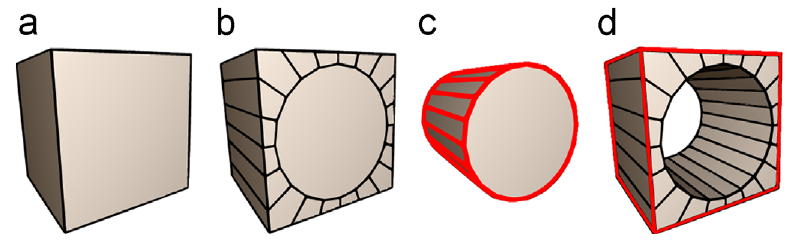
\includegraphics[width=13cm]{figuras/convex_polyhedra.png}
	}
	{\Fonte{\cite{fellner2013}}}	
\end{figure}

As \textit{deformation grammars}, por sua vez, foram introduzidas por \citeonline{vimont2017}, permitindo deformar livremente objetos complexos ou conjuntos de objetos, preservando sua consistência. Elas processam deformações de objetos como símbolos, graças às regras de interpretação definidas pelo usuário. Um exemplo é mostrado na Figura \ref{fig:vimont}.

\begin{figure}[h!]
	\centering
	\captionsetup{width=15cm}
	\Caption{\label{fig:vimont} O modelo inicial de uma casa (a) é deformado pelo usuário enquanto preserva as propriedades típicas, como a ortogonalidade da parede e a disposição linear do piso (b).}
	\UFCfig{}{
		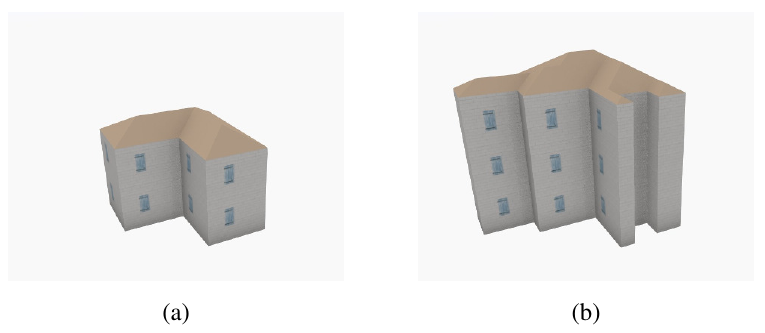
\includegraphics[width=13cm]{figuras/deformation_grammar.png}
	}
	{\Fonte{\cite{vimont2017}}}	
\end{figure}